% ******************************* Thesis Appendix A ****************************
\chapter{Supporting figures to Monte Carlo studies concerning determining interaction times using the effects of diffusion} ~\label{sec:DiffMCPlots}

\graphicspath{{Appendix1/Figs/PDF/}{Appendix1/Figs/Raster/}{Appendix1/Figs/Vector/}}

The following figures support the figures shown in Section~\ref{sec:DiffMCStudies}.

Figures~\ref{fig:DiffNoiseStudy_HitFit},~\ref{fig:DiffNoiseStudy_CDiff4},~\ref{fig:DiffNoiseStudy_RMS0cm}, and~\ref{fig:DiffNoiseStudy_ChargeCut} correspond to changing levels of the electronics noise.

Figures~\ref{fig:DiffLifeStudy_HitFit},~\ref{fig:DiffLifeStudy_CDiff4},~\ref{fig:DiffLifeStudy_RMS0cm}, and~\ref{fig:DiffLifeStudy_ChargeCut} correspond to changing electron lifetimes.

Figures~\ref{fig:DiffElecStudy_HitFit},~\ref{fig:DiffElecStudy_CDiff4},~\ref{fig:DiffElecStudy_RMS0cm}, and~\ref{fig:DiffElecStudy_ChargeCut} correspond to changing electric fields.

Figures~\ref{fig:DiffLDiff_HitFit},~\ref{fig:DiffLDiff_CDiff4},~\ref{fig:DiffLDiff_RMS0cm}, and~\ref{fig:DiffLDiff_ChargeCut} correspond to changing constants of longitudinal diffusion. \\

Figures~\ref{fig:DiffNoiseStudy_HitFit},~\ref{fig:DiffLifeStudy_HitFit},~\ref{fig:DiffElecStudy_HitFit}, and~\ref{fig:DiffLDiff_HitFit} show how the distributions of the hit $RMS$ and hit $RMS/Charge$ change for hits between 20 and 30 cm from the APAs.

Figures~\ref{fig:DiffNoiseStudy_CDiff4},~\ref{fig:DiffLifeStudy_CDiff4},~\ref{fig:DiffElecStudy_CDiff4}, and~\ref{fig:DiffLDiff_CDiff4} show how the most probable values of hit $RMS$ changes with drift distance for tracks associated with counter differences of 4.

Figures~\ref{fig:DiffNoiseStudy_RMS0cm},~\ref{fig:DiffLifeStudy_RMS0cm},~\ref{fig:DiffElecStudy_RMS0cm}, and~\ref{fig:DiffLDiff_RMS0cm} show how the most probable value of hit $RMS$ next to the APAs changes with increasing counter difference.

Figures~\ref{fig:DiffNoiseStudy_ChargeCut},~\ref{fig:DiffLifeStudy_ChargeCut},~\ref{fig:DiffElecStudy_ChargeCut}, and~\ref{fig:DiffLDiff_ChargeCut} show the normalised hit charge distributions for increasing noise levels, and the cut which is applied to remove the tails of the distribution. \\ 

%%%%%%%% The electronics noise study
\begin{figure}
  \centering
  \begin{subfigure}{0.48\textwidth}
    \centering
    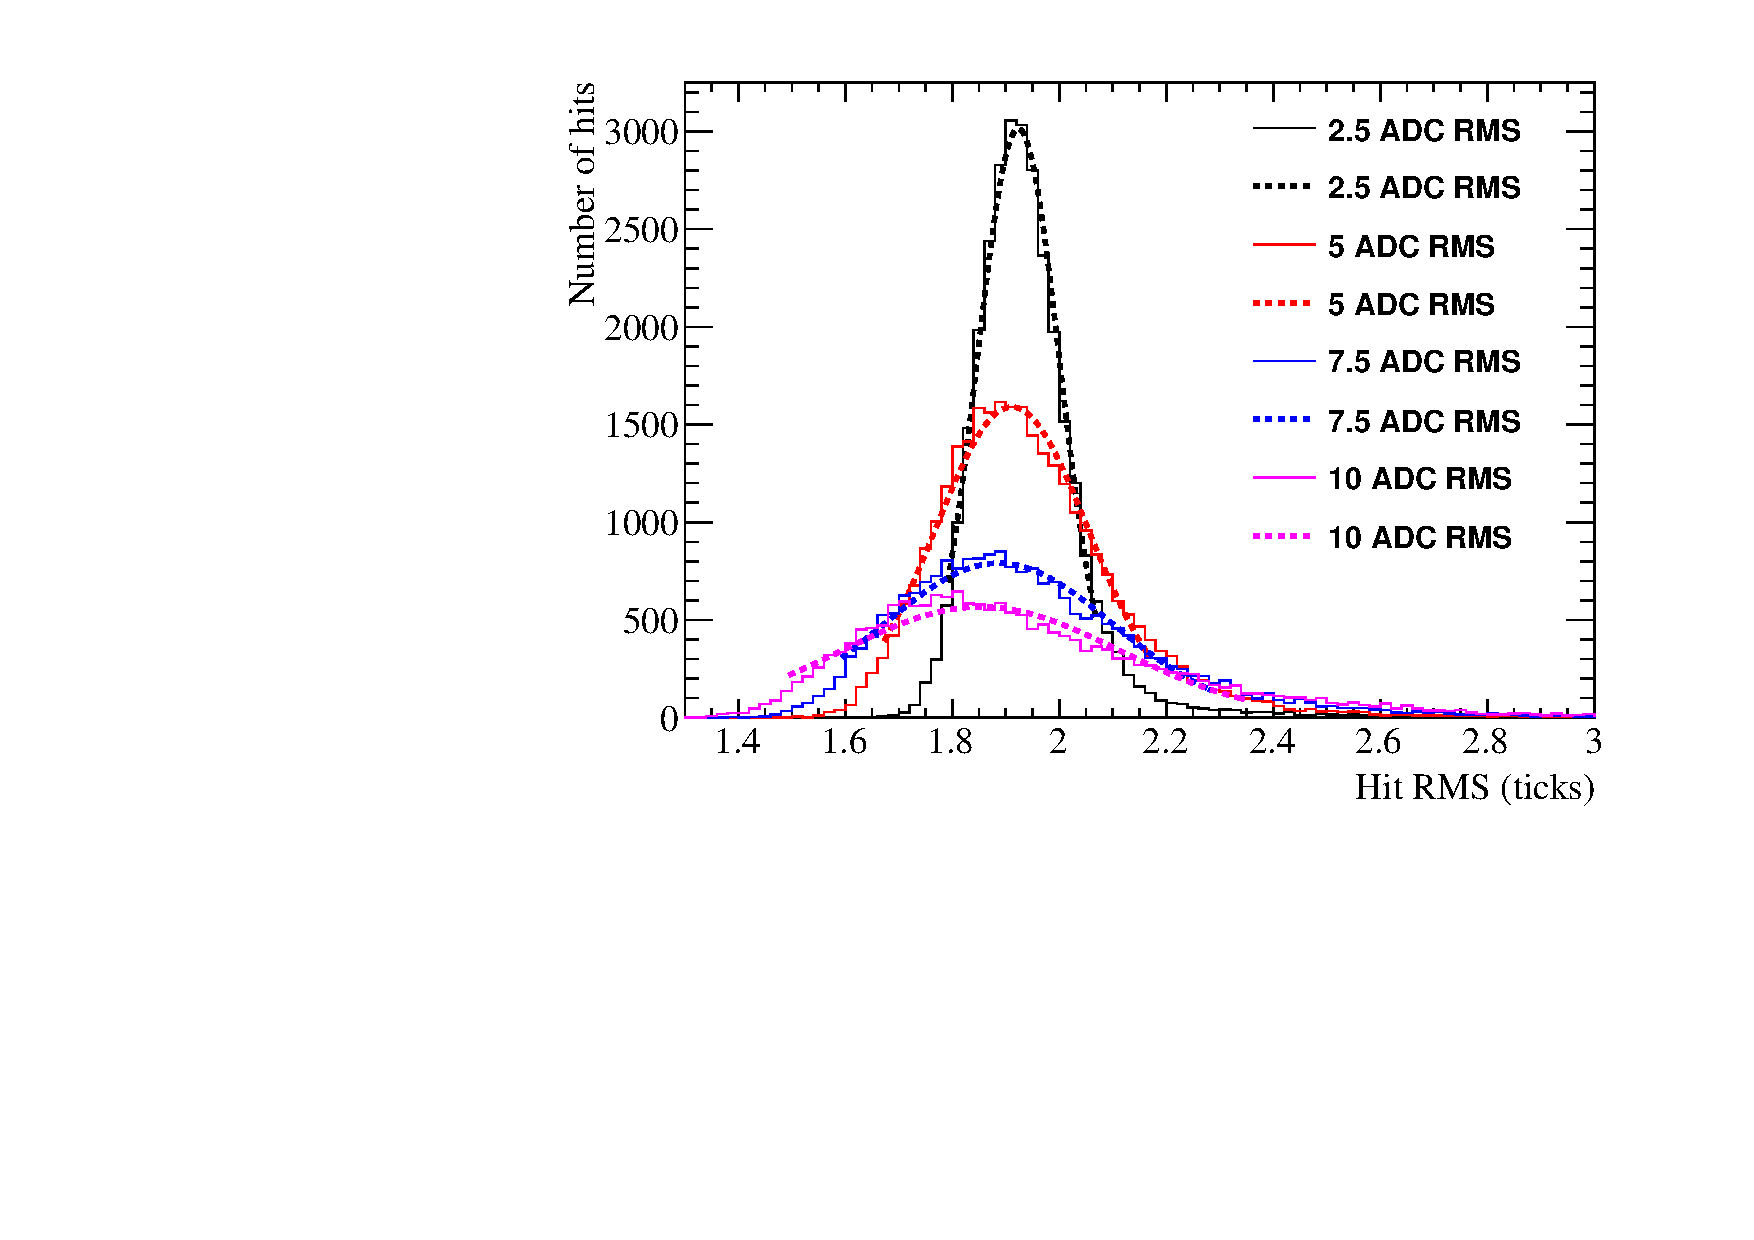
\includegraphics[width=\textwidth]{Canvas_RMS_20cm_NoiseLevel}
    \caption{The distribution of hit $RMS$ values for hits between $x =$ 20 cm and $x =$ 30 cm.}
  \end{subfigure}%
  \hspace{0.03\textwidth}%
  \begin{subfigure}{0.48\textwidth}
    \centering
    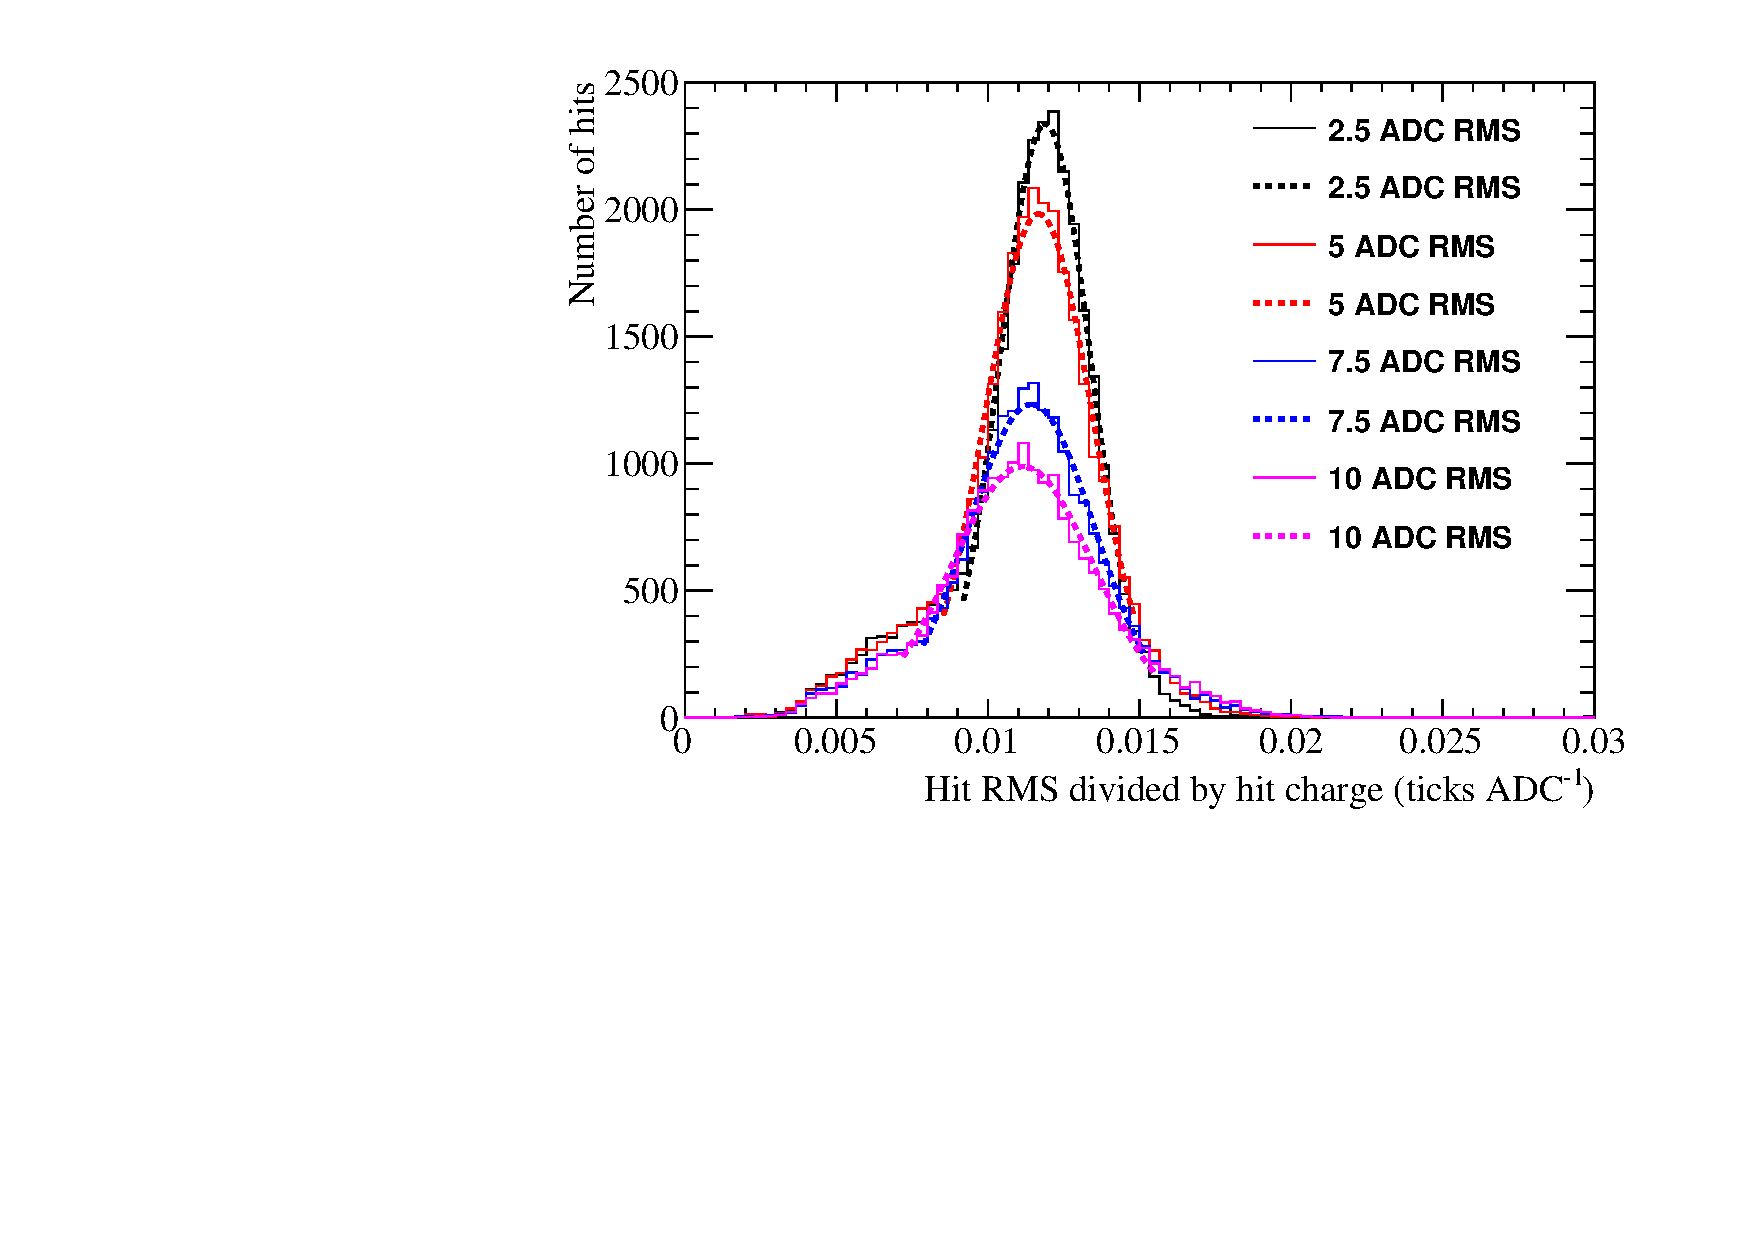
\includegraphics[width=\textwidth]{Canvas_RMS_Q_20cm_NoiseLevel}
    \caption{The distribution of hit $RMS/Charge$ values for hits between $x =$ 20 cm and $x =$ 30 cm.}
  \end{subfigure}
  \caption[The distributions of the hit $RMS$ and hit $RMS/Charge$ values for tracks with a counter difference of 4, for different values of the electronics noise]
          {The distributions of the hit $RMS$ and hit $RMS/Charge$ values for hits between $x$~=~20~cm and $x$~=~30~cm, for tracks with a counter difference of 4, for different values of the electronics noise.}
  \label{fig:DiffNoiseStudy_HitFit}
\end{figure}

\begin{figure}
  \centering
  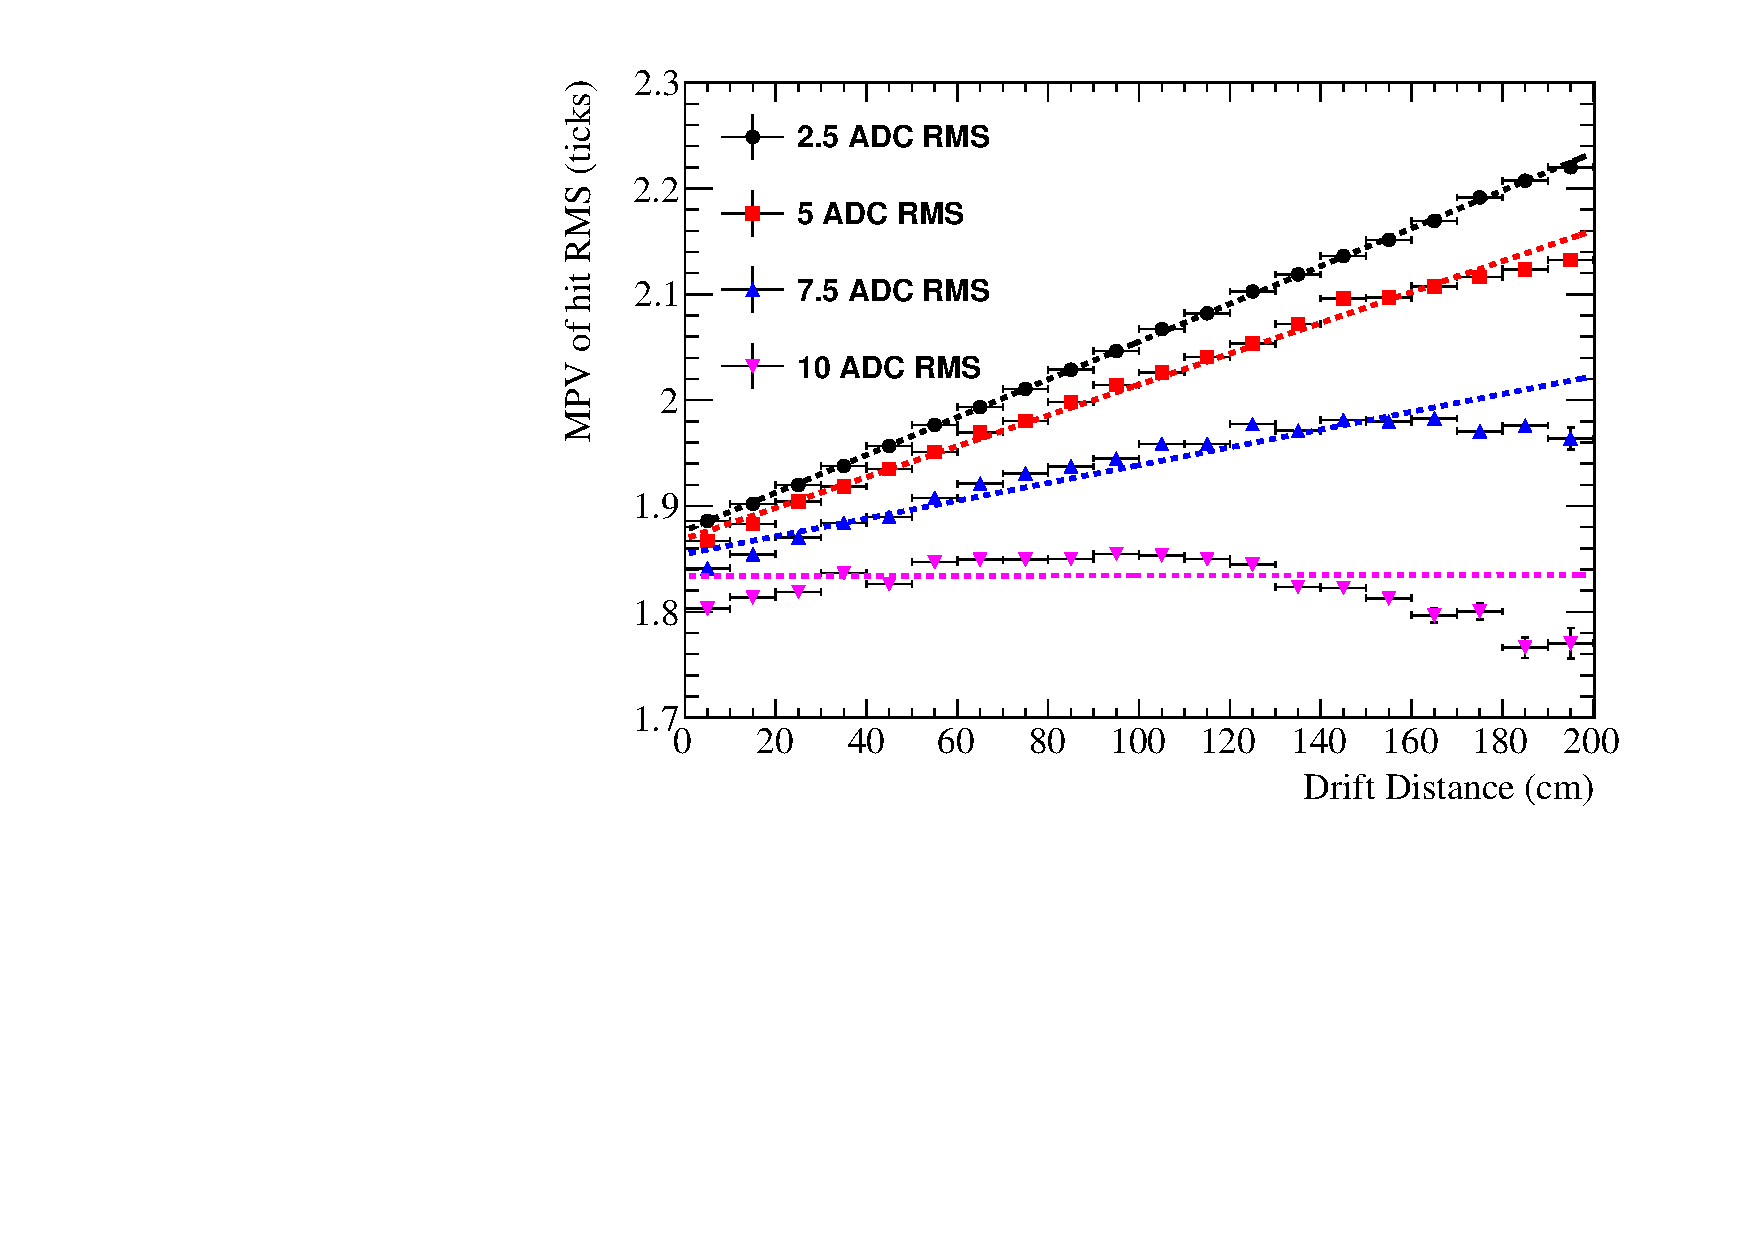
\includegraphics[width=0.6\textwidth]{Canvas_CountDiff4_All_Positions_NoiseLevel}
  \caption[The most probable values of hit $RMS$ as a function of drift distance, for tracks associated with a coincidence that had a counter difference of 4, for different values of the electronics noise]
          {The most probable values of hit $RMS$ as a function of drift distance, for tracks associated with a coincidence that had a counter difference of 4, for different values of the electronics noise.}
  \label{fig:DiffNoiseStudy_CDiff4}
\end{figure}

\begin{figure}
  \centering
  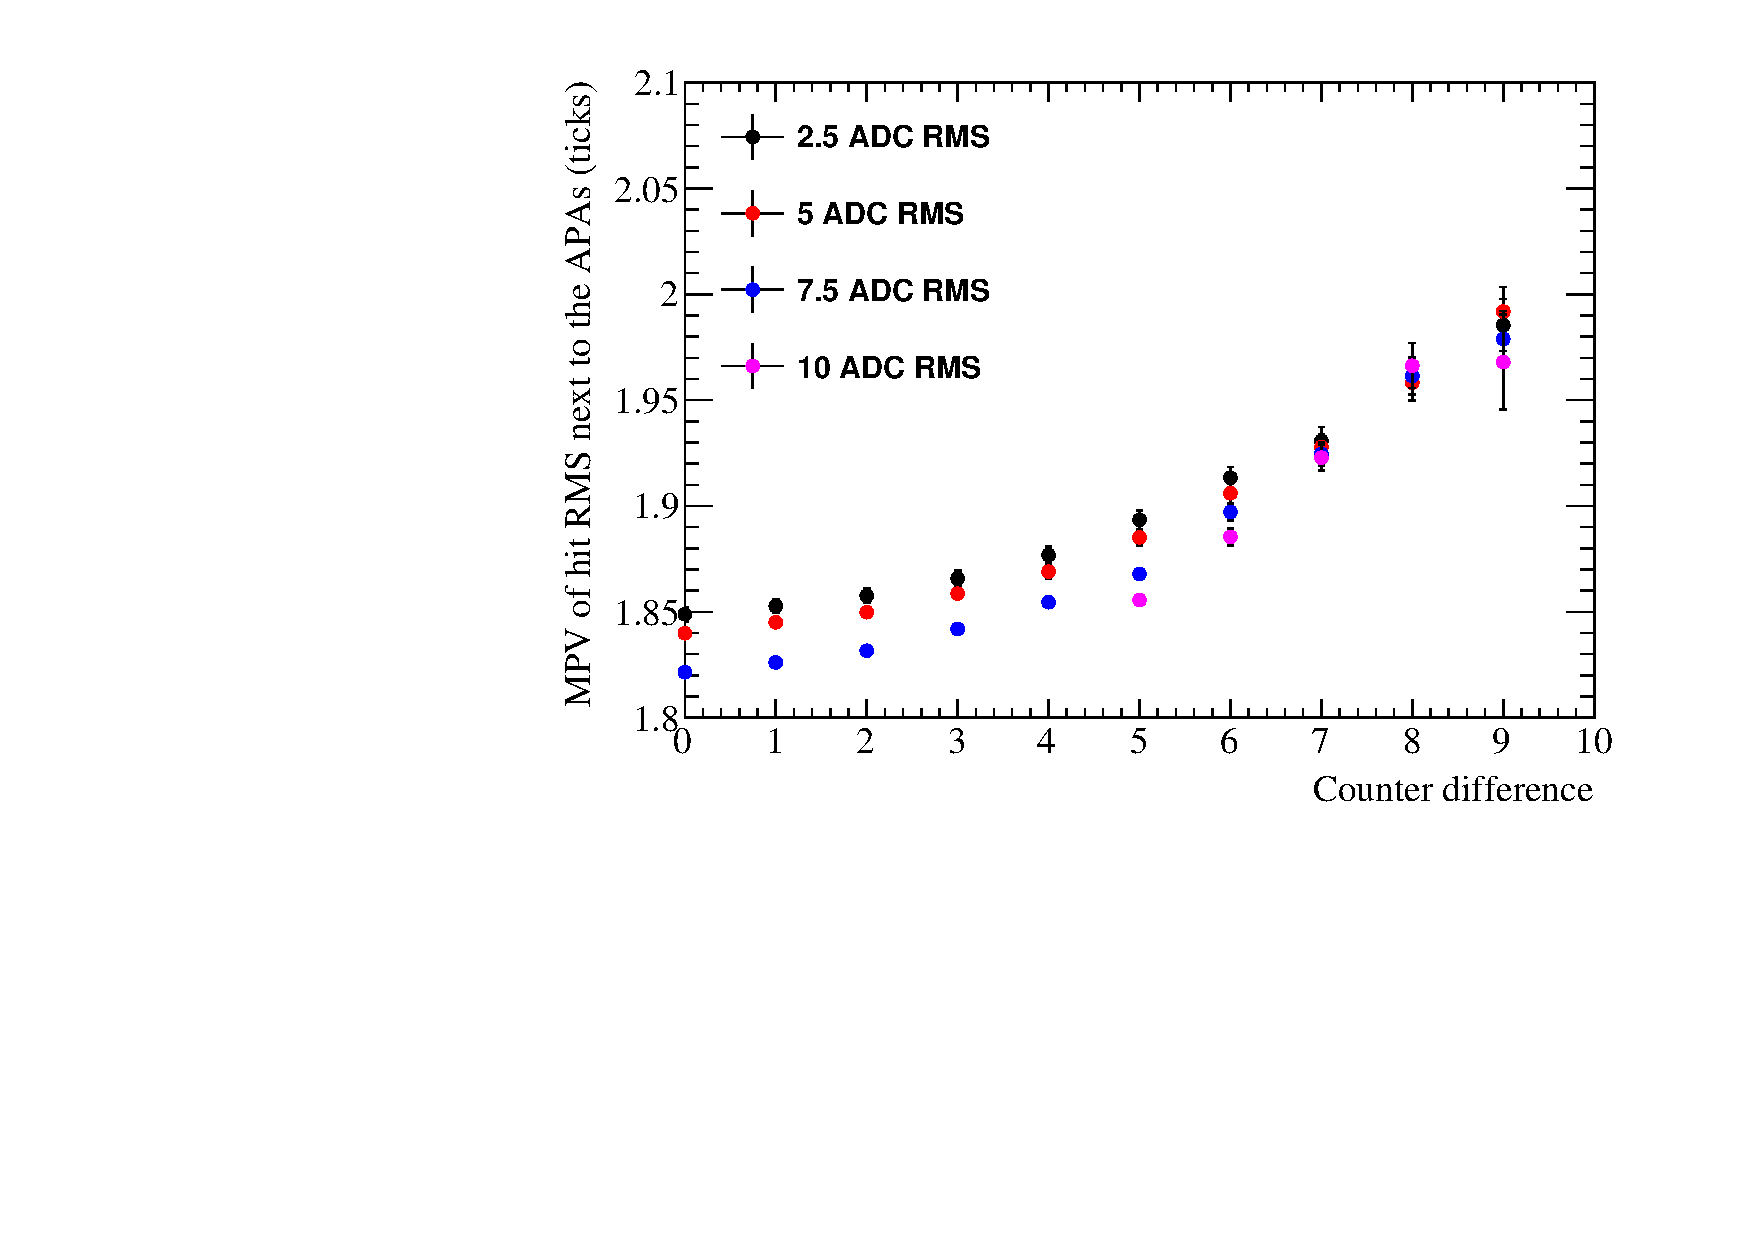
\includegraphics[width=0.6\textwidth]{Canvas_All_Angles_RMS0cm_NoiseLevel}
  \caption[The angular dependence of hits within 10 cm of the APAs, for different values of the electronics noise]
          {The most probable values of hit $RMS$ within 10 cm of the APAs, as a function of the counter difference of the coincidence that the track was associated with, for different values of the electronics noise.}
  \label{fig:DiffNoiseStudy_RMS0cm}
\end{figure}

\begin{figure}
  \centering
  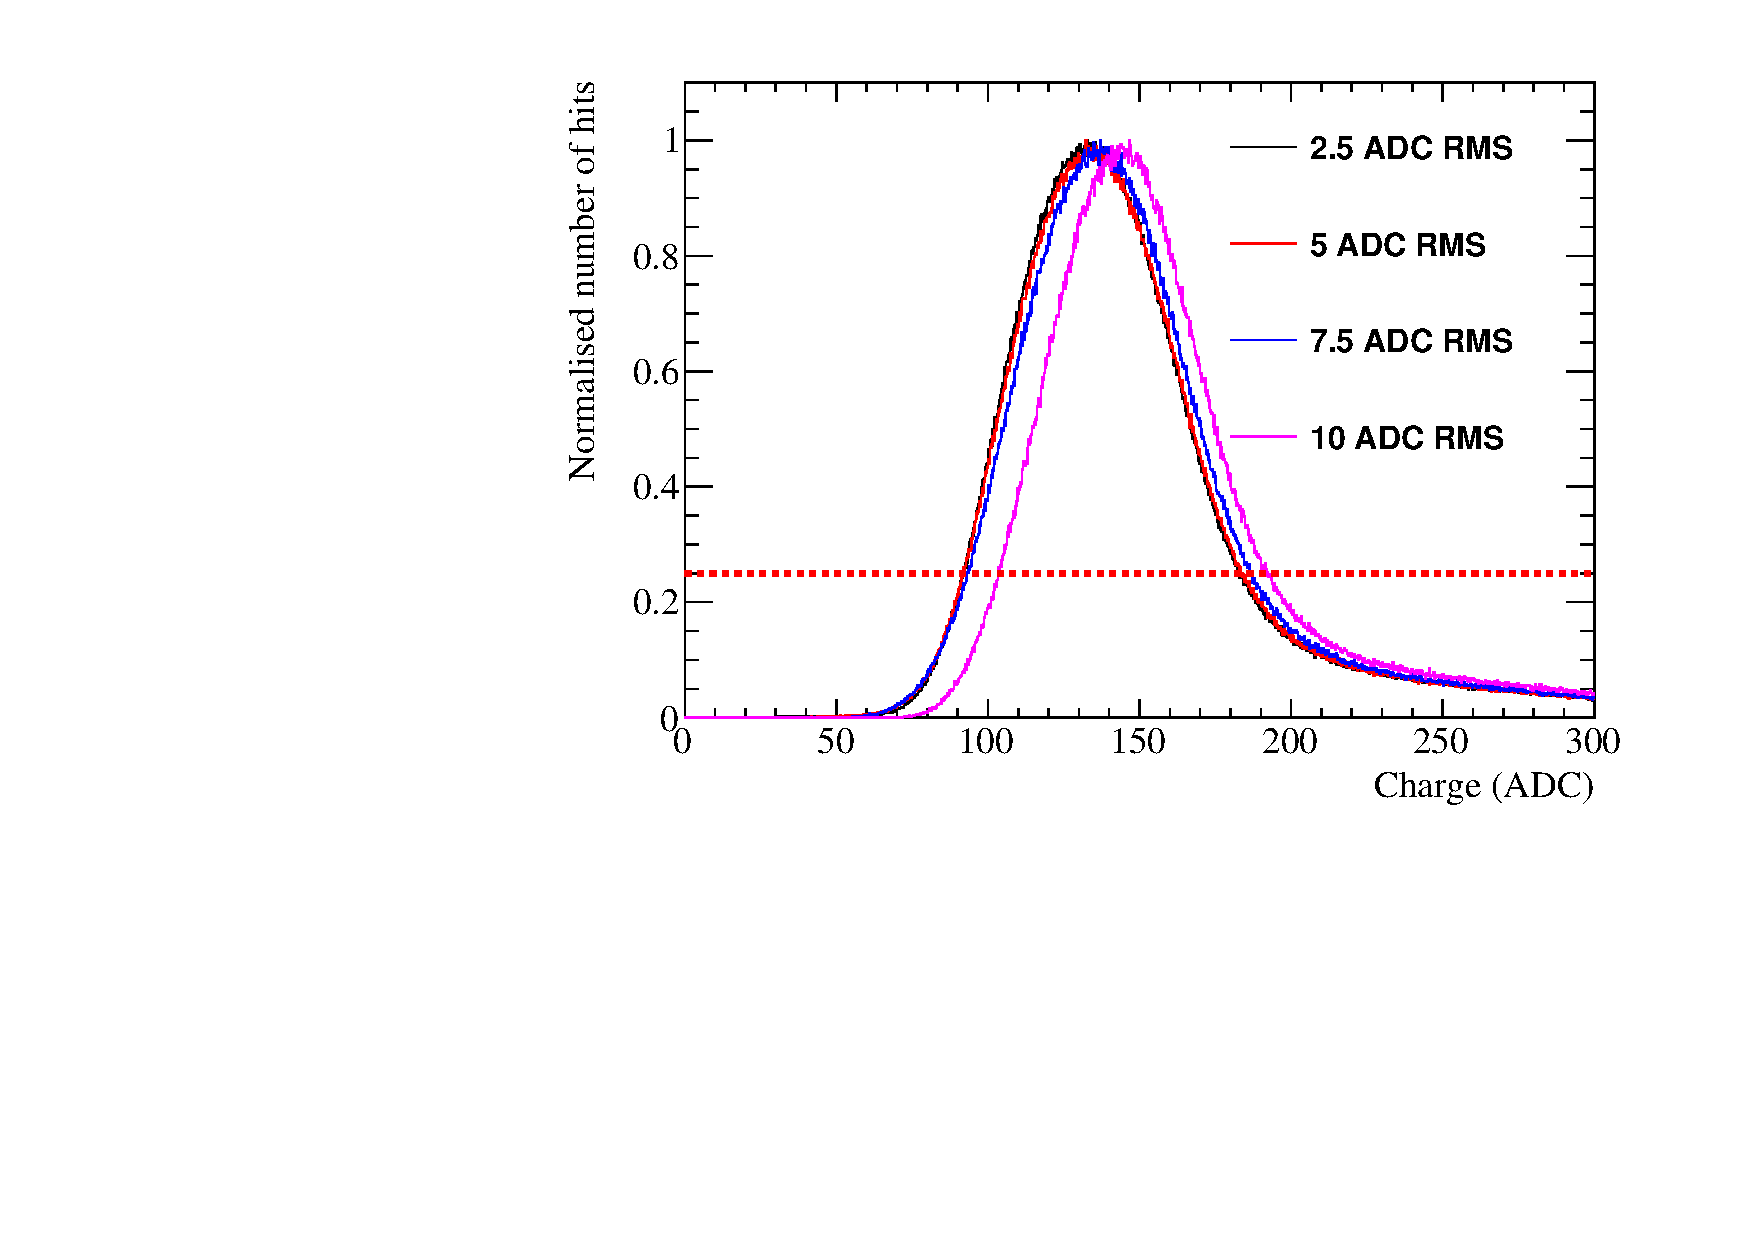
\includegraphics[width=0.6\textwidth]{Canvas_ChargeCut_NoiseLevel}
  \caption[The normalised hit charge distribution for different values of the electronics noise]
          {The normalised hit charge distribution for different values of the electronics noise. The hit charge is shown in units of ADC, and is normalised so that the most common hit charge has a value of 1. A cut on the normalised number of hits being greater than 0.25 is shown, the aim of this cut is to remove the tails of the hit charge distribution.}
  \label{fig:DiffNoiseStudy_ChargeCut}
\end{figure}

%%%%%%%% The Electron lifetime study

\begin{figure}
  \centering
  \begin{subfigure}{0.48\textwidth}
    \centering
    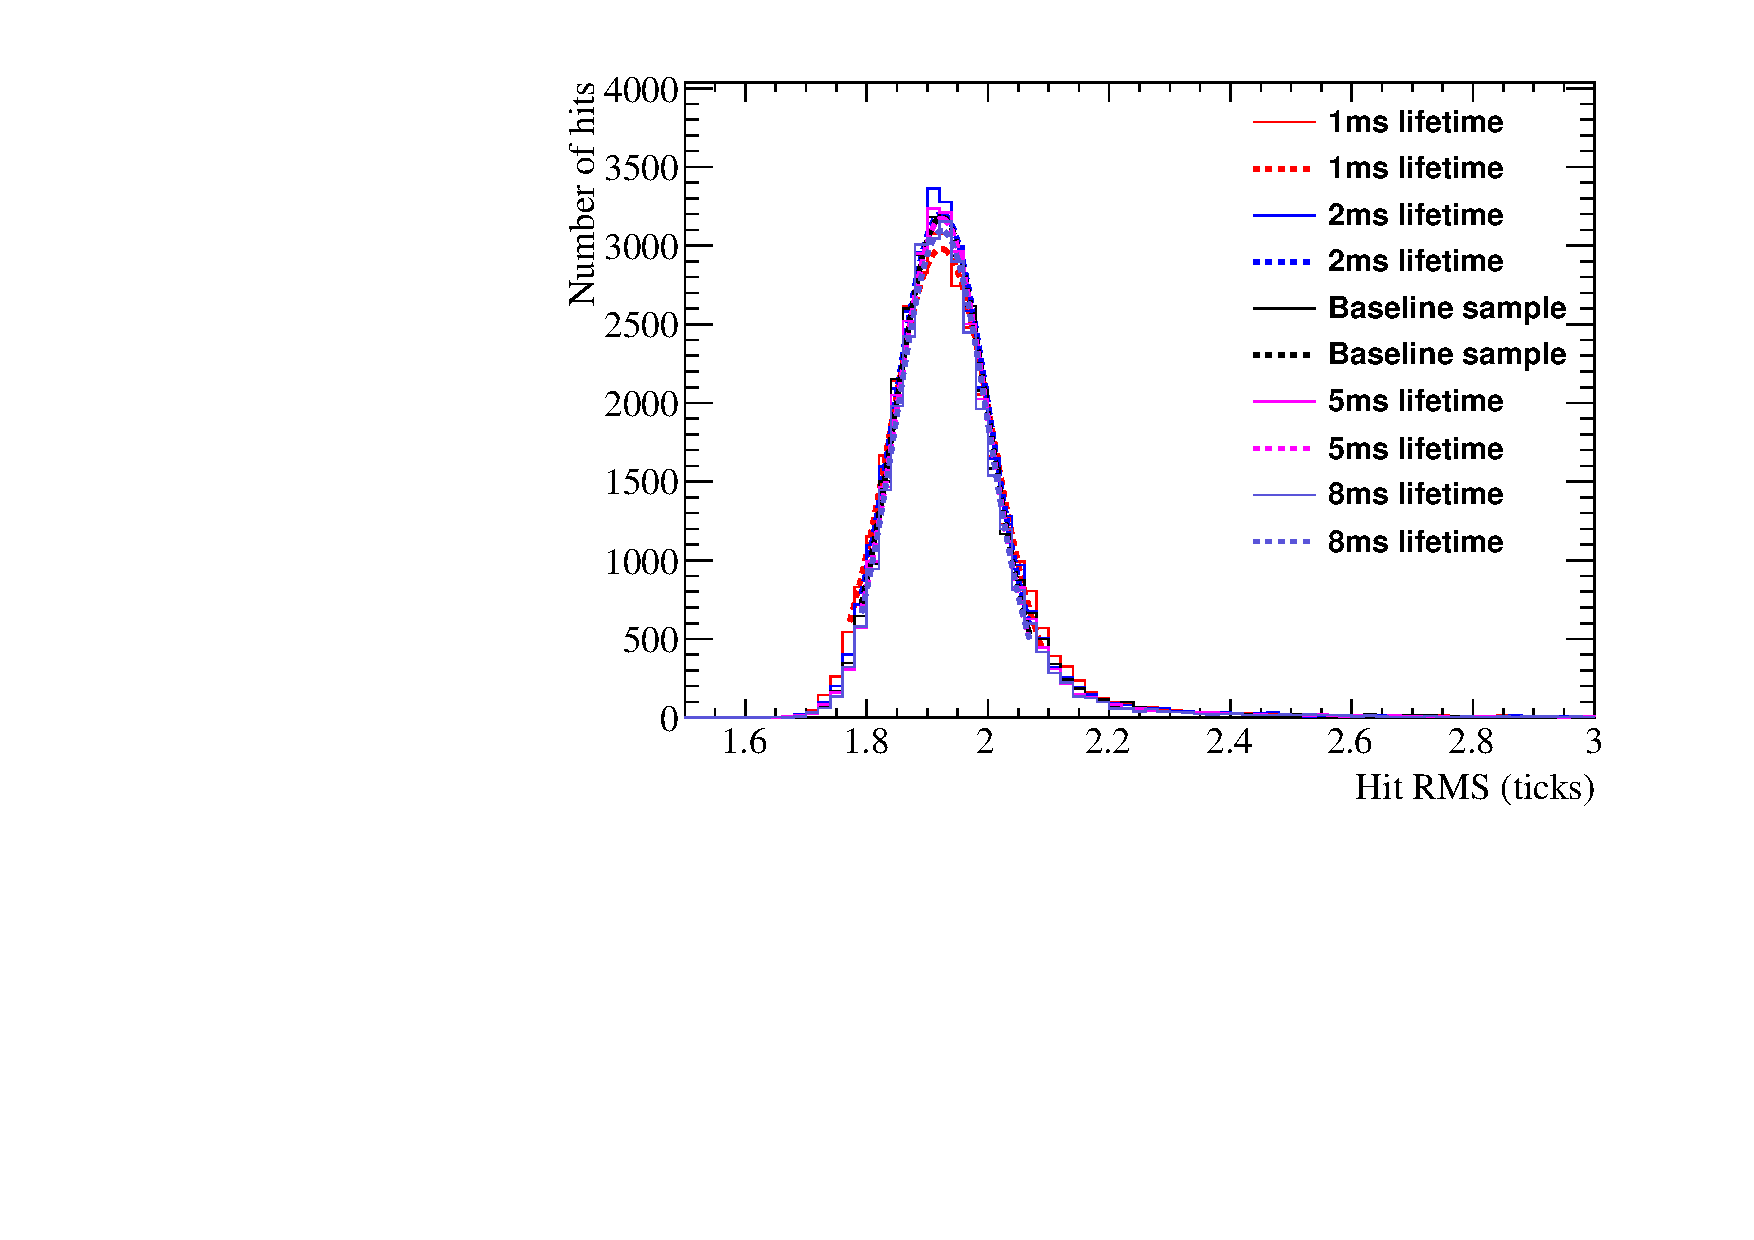
\includegraphics[width=\textwidth]{Canvas_RMS_20cm_ElecLifetime}
    \caption{The distribution of hit $RMS$ values for hits between $x =$ 20 cm and $x =$ 30 cm.}
  \end{subfigure}%
  \hspace{0.03\textwidth}%
  \begin{subfigure}{0.48\textwidth}
    \centering
    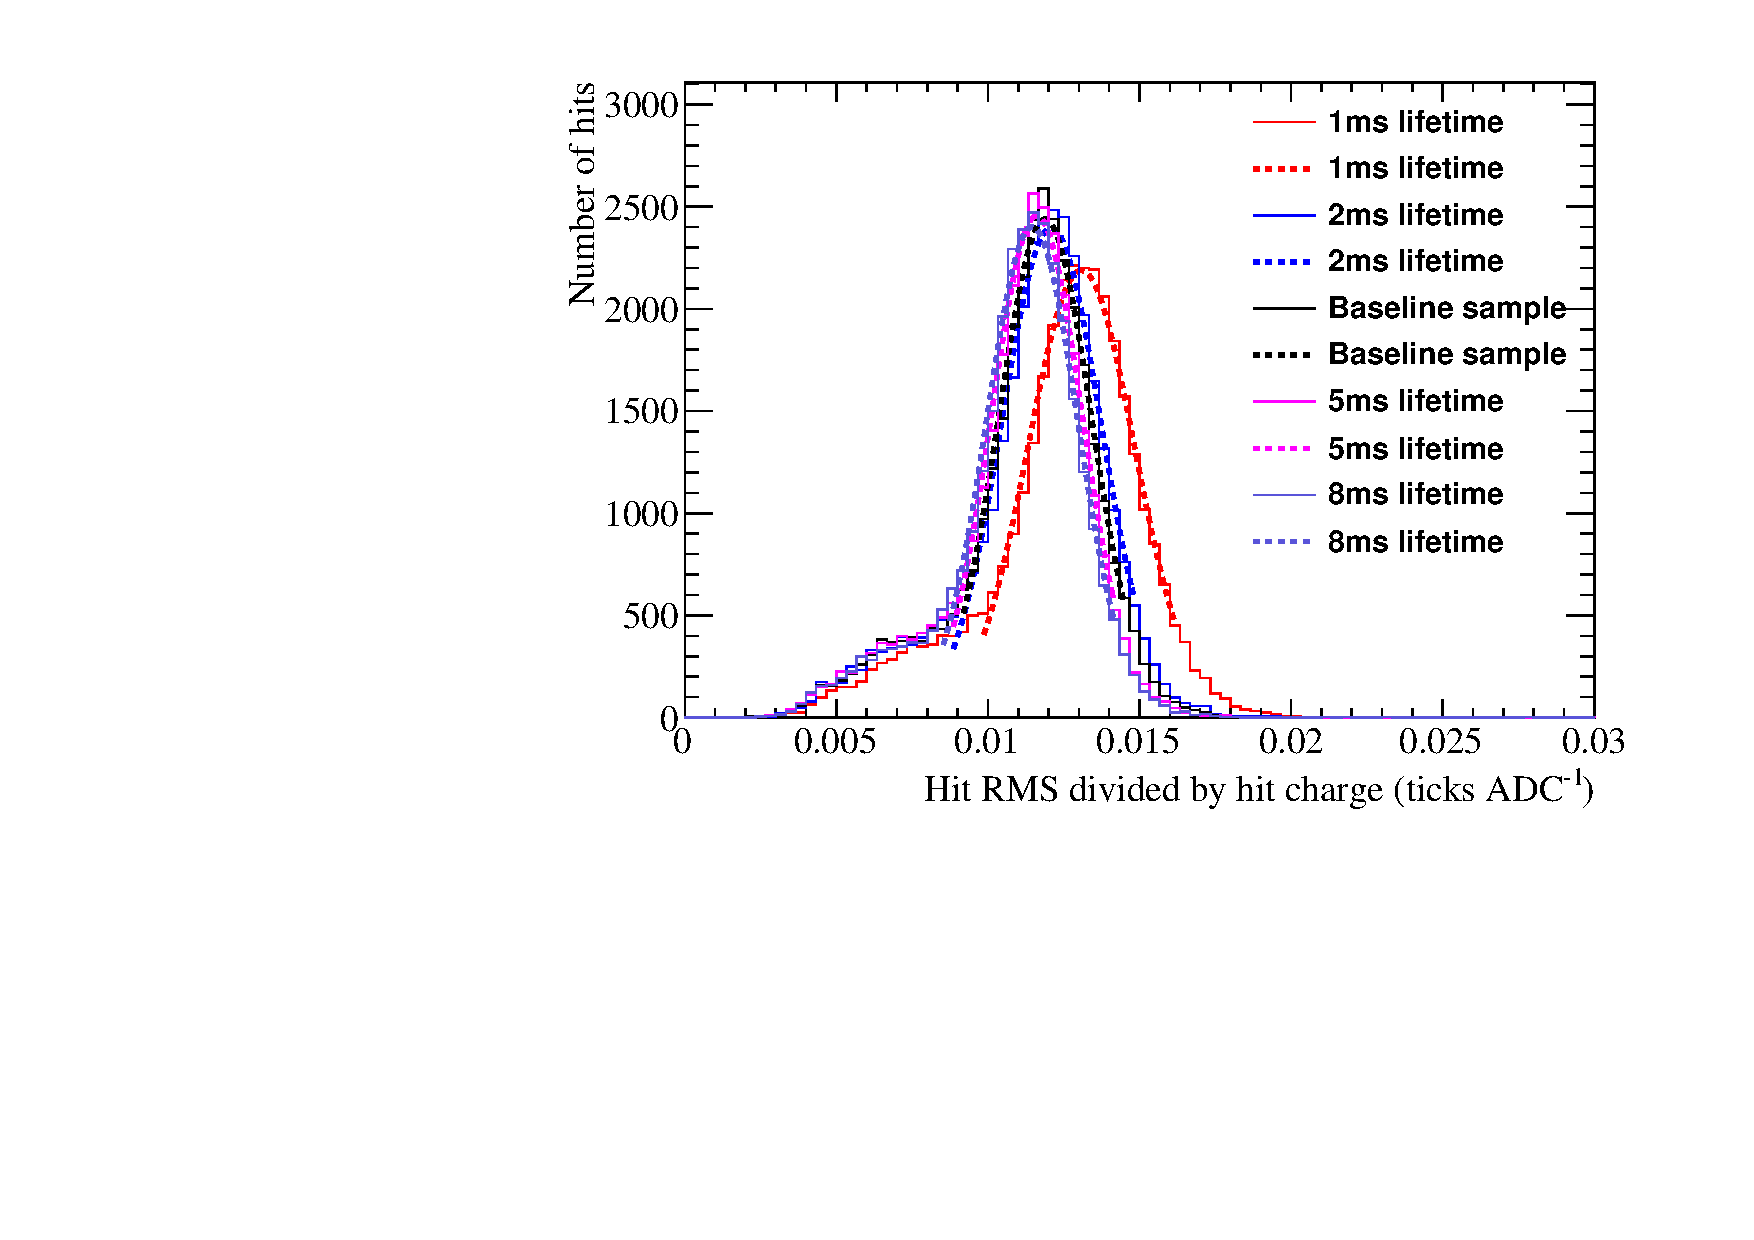
\includegraphics[width=\textwidth]{Canvas_RMS_Q_20cm_ElecLifetime}
    \caption{The distribution of hit $RMS/Charge$ values for hits between $x =$ 20 cm and $x =$ 30 cm.}
  \end{subfigure}
  \caption[The distributions of the hit $RMS$ and hit $RMS/Charge$ values for tracks with a counter difference of 4, for different values of the electron lifetime]
          {The distributions of the hit $RMS$ and hit $RMS/Charge$ values for hits between $x$~=~20~cm and $x$~=~30~cm, for tracks with a counter difference of 4, for different values of the electron lifetime.}
  \label{fig:DiffLifeStudy_HitFit}
\end{figure}

\begin{figure}
  \centering
  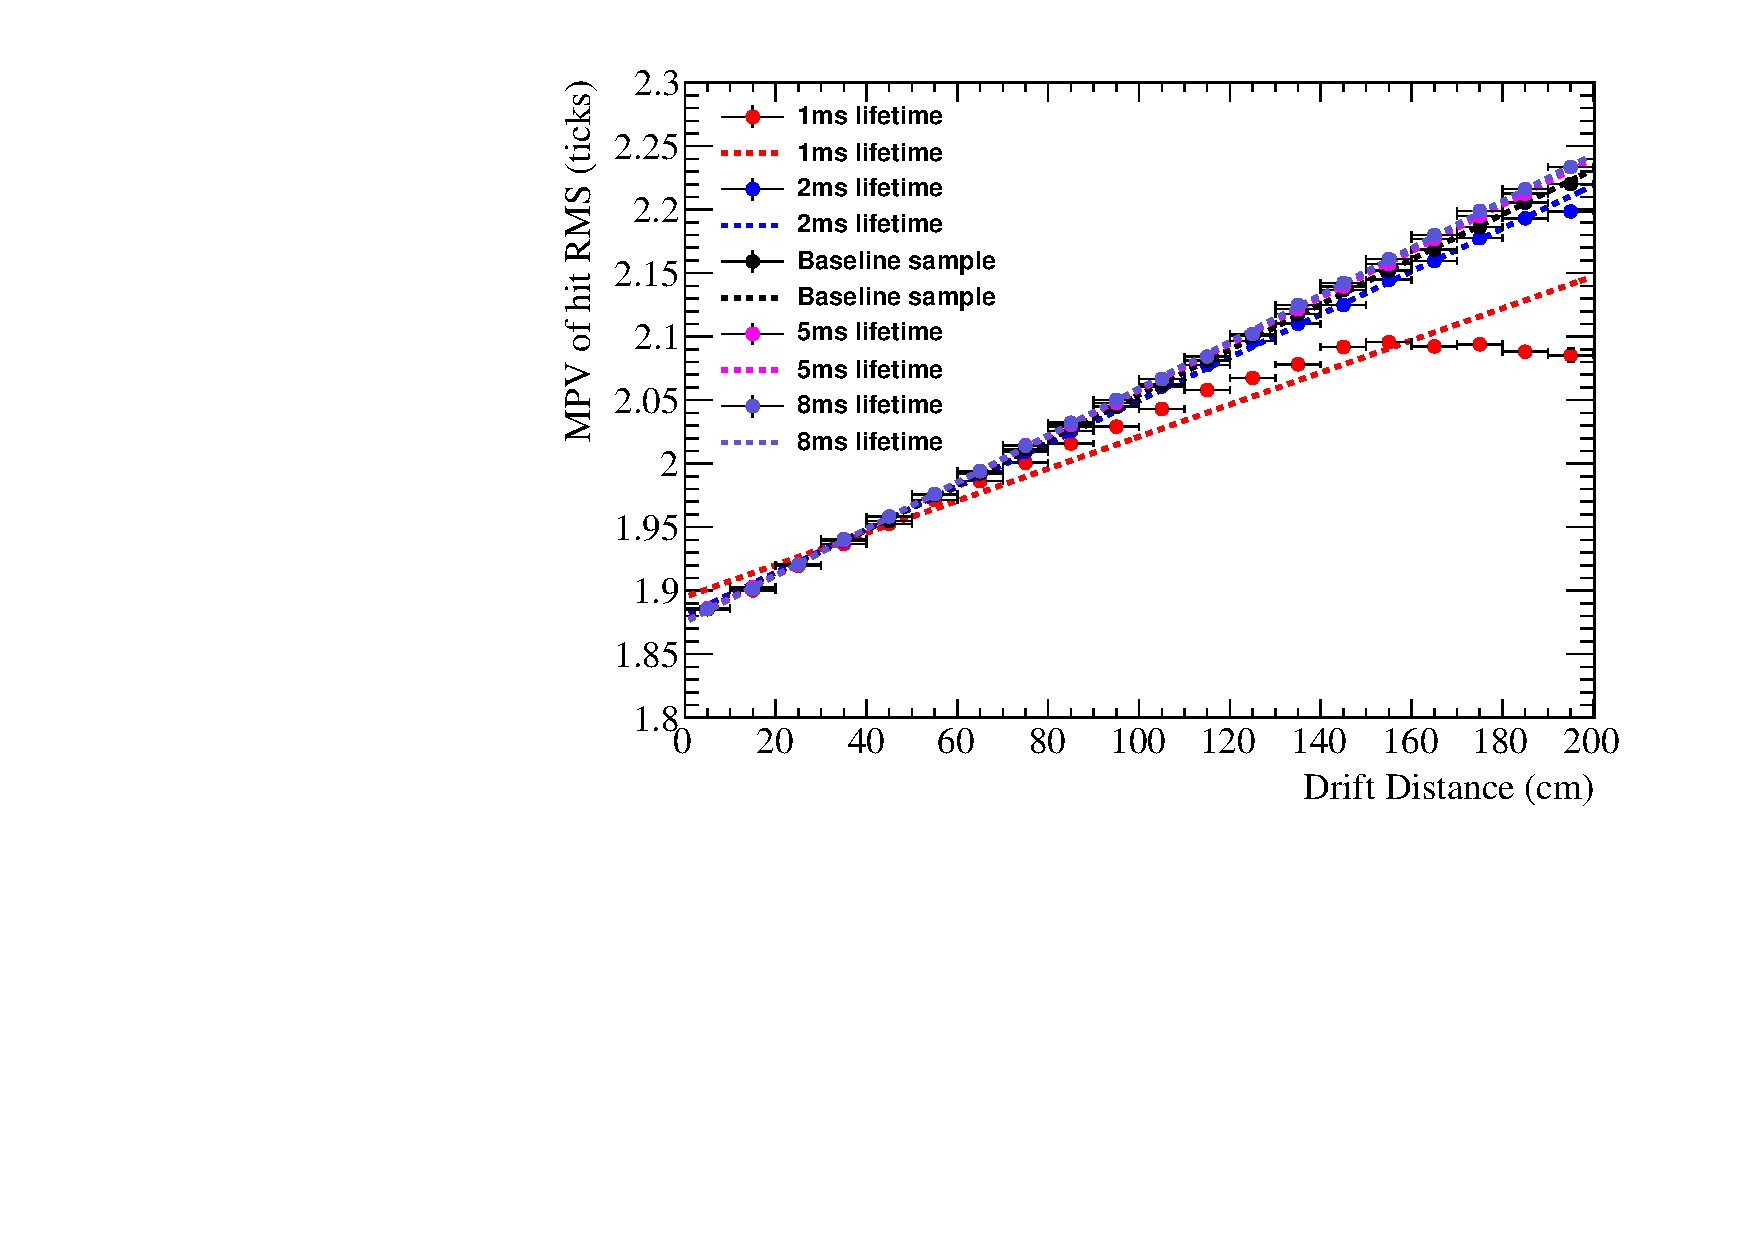
\includegraphics[width=0.6\textwidth]{Canvas_CountDiff4_All_Positions_ElecLifetime}
  \caption[The most probable values of hit $RMS$ as a function of drift distance, for tracks associated with a coincidence that had a counter difference of 4, for different values of the electron lifetime]
          {The most probable values of hit $RMS$ as a function of drift distance, for tracks associated with a coincidence that had a counter difference of 4, for different values of the electron lifetime.}
  \label{fig:DiffLifeStudy_CDiff4}
\end{figure}

\begin{figure}
  \centering
  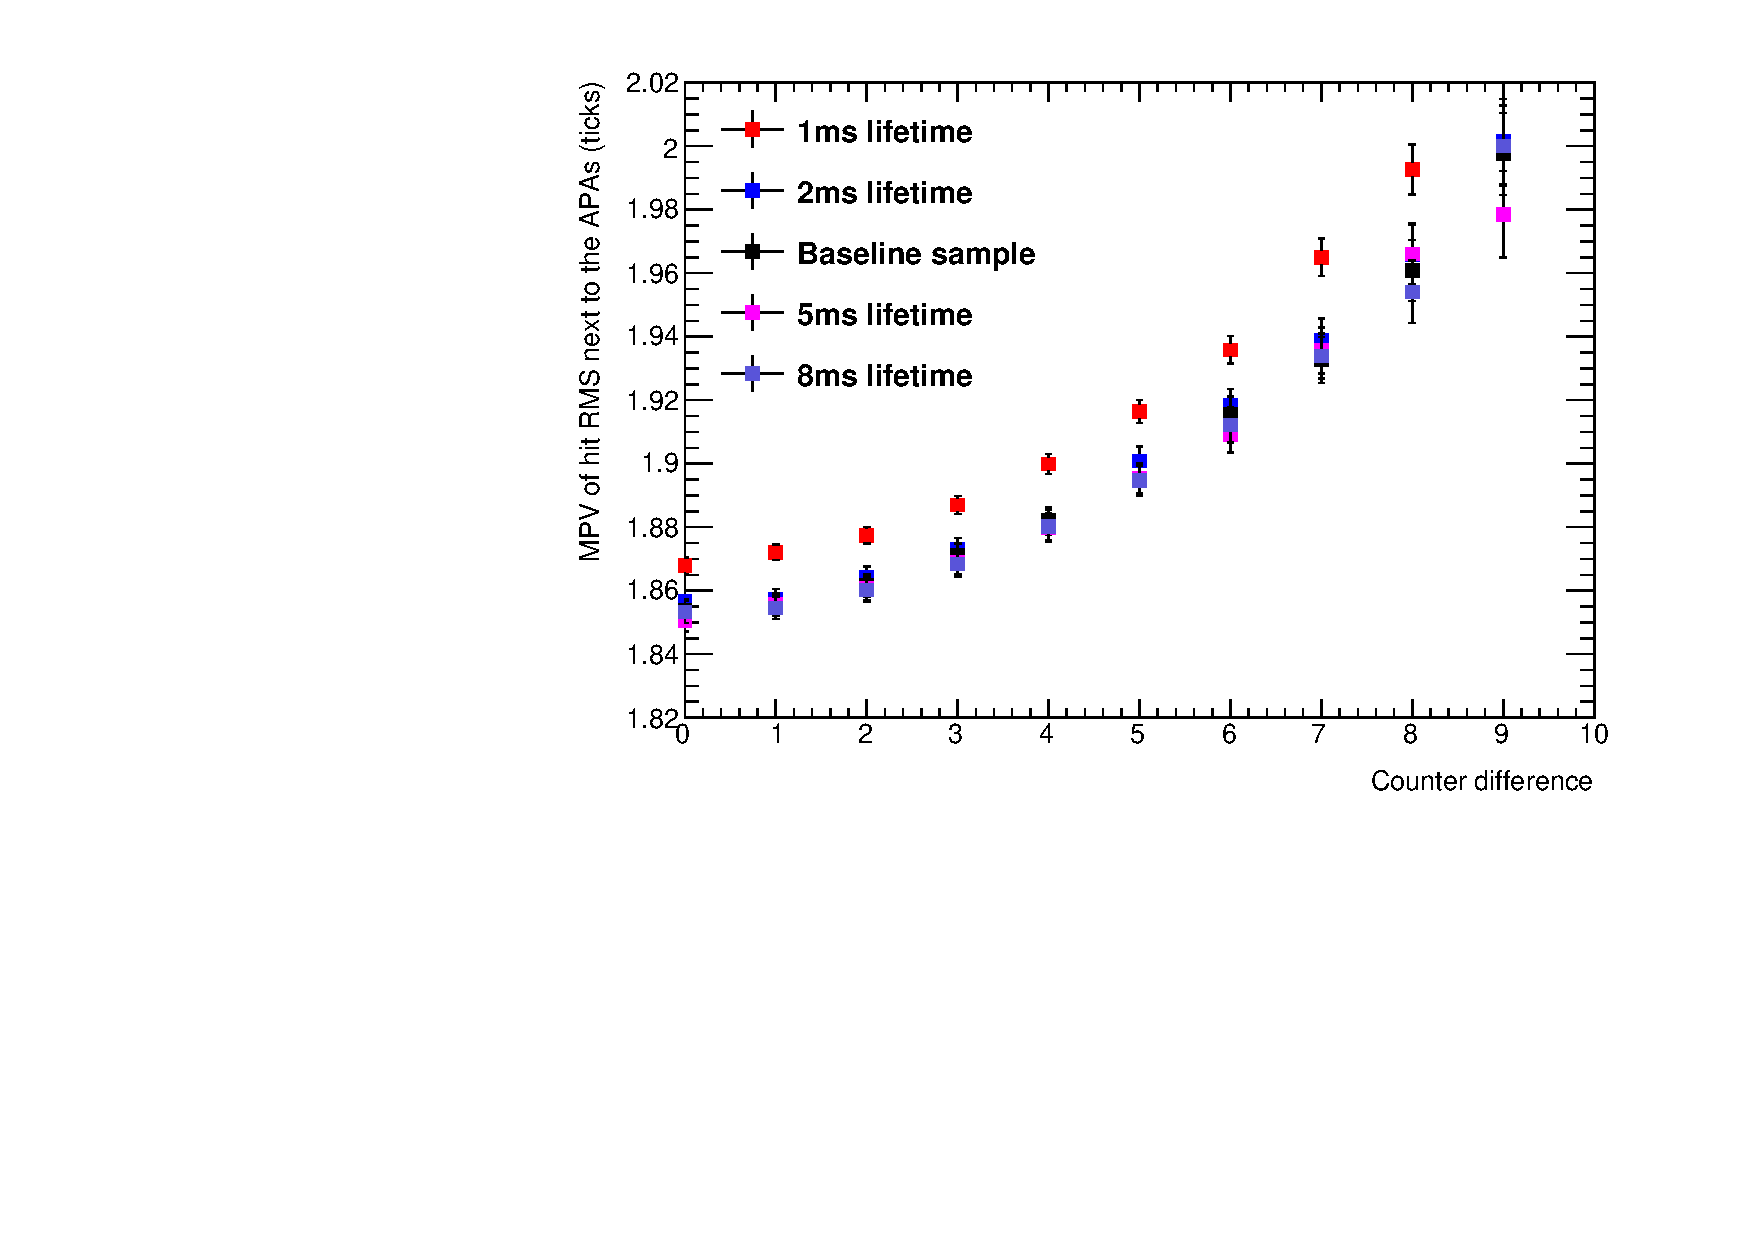
\includegraphics[width=0.6\textwidth]{Canvas_All_Angles_RMS0cm_ElecLifetime}
    \caption[The angular dependence of hits within 10 cm of the APAs, for different values of the electron lifetime]
            {The most probable values of hit $RMS$ within 10 cm of the APAs, as a function of the counter difference of the coincidence that the track was associated with, for different values of the electron lifetime.}
  \label{fig:DiffLifeStudy_RMS0cm}
\end{figure}

\begin{figure}
  \centering
  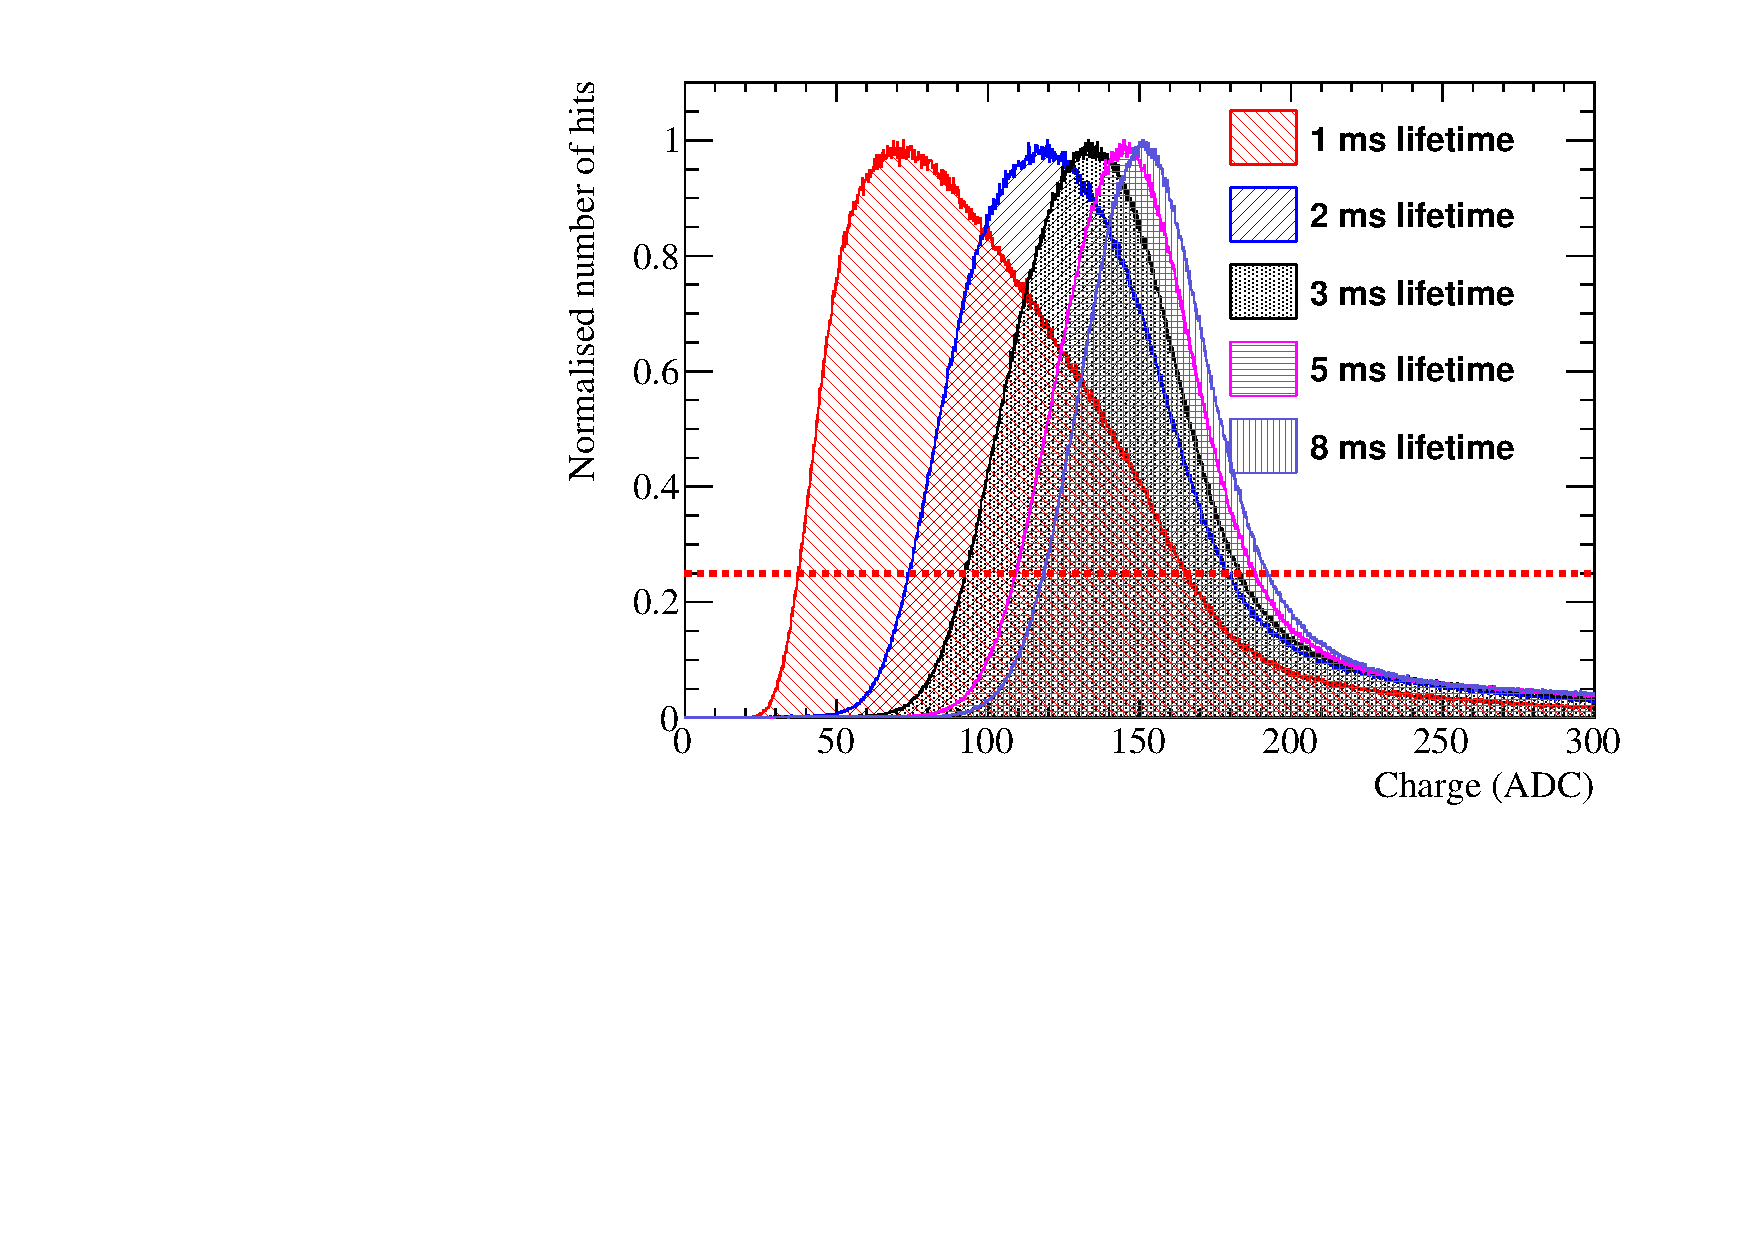
\includegraphics[width=0.6\textwidth]{Canvas_ChargeCut_ElecLifetime}
  \caption[The normalised hit charge distribution for different values of the electron lifetime]
          {The normalised hit charge distribution for different values of the electron lifetime. The hit charge is shown in units of ADC, and is normalised so that the most common hit charge has a value of 1. A cut on the normalised number of hits being greater than 0.25 is shown, the aim of this cut is to remove the tails of the hit charge distribution.}
  \label{fig:DiffLifeStudy_ChargeCut}
\end{figure}

%%%%%%%% The Electric field study

\begin{figure}
  \centering
  \begin{subfigure}{0.48\textwidth}
    \centering
    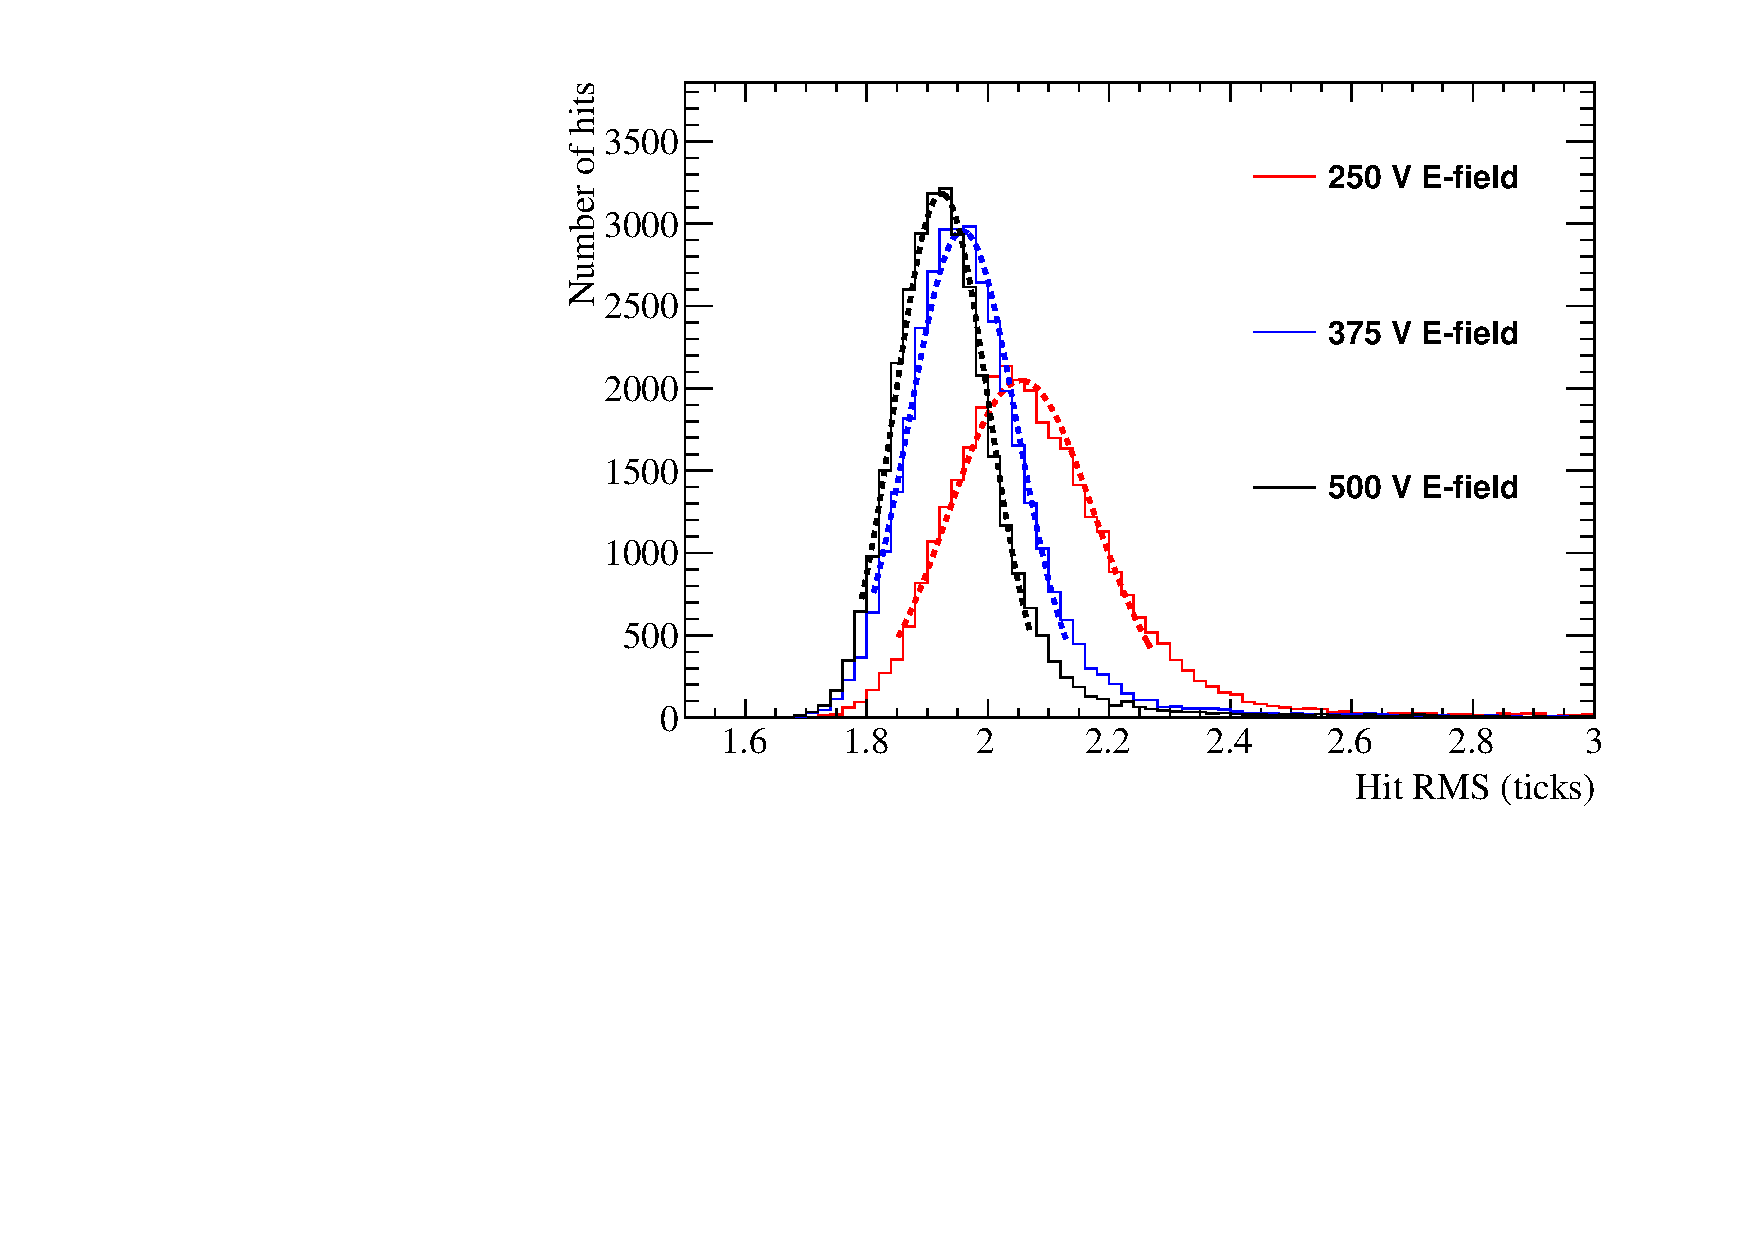
\includegraphics[width=\textwidth]{Canvas_RMS_20cm_ElecField}
    \caption{The most probable hit $RMS$ values for hits between $x =$ 20 cm and $x =$ 30 cm.}
  \end{subfigure}%
  \hspace{0.03\textwidth}%
  \begin{subfigure}{0.48\textwidth}
    \centering
    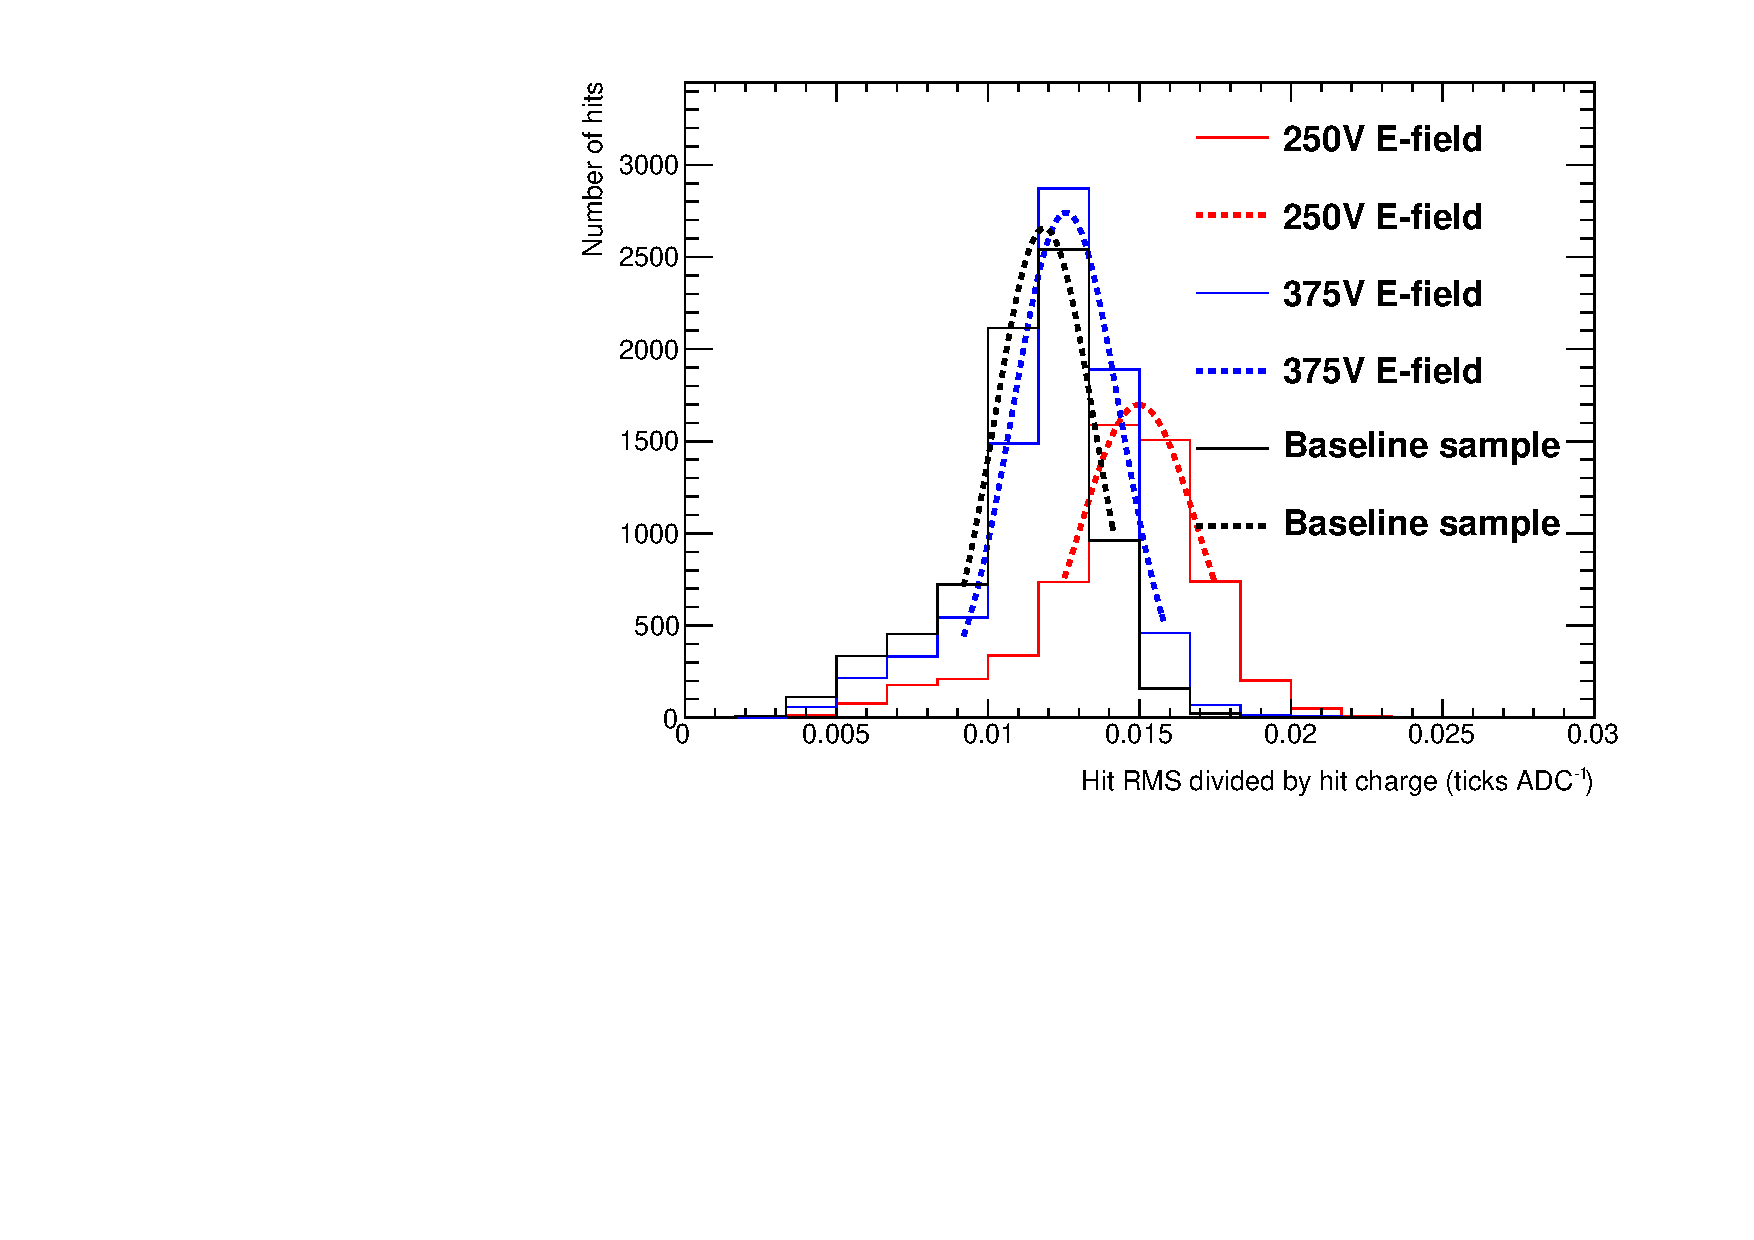
\includegraphics[width=\textwidth]{Canvas_RMS_Q_20cm_ElecField}
    \caption{The most probably hit $RMS/Charge$ values for hits between $x =$ 20 cm and $x =$ 30 cm.}
  \end{subfigure}
  \caption[The distributions of the hit $RMS$ and hit $RMS/Charge$ values for tracks with a counter difference of 4, for different values of the electric field]
          {The distributions of the hit $RMS$ and hit $RMS/Charge$ values for hits between $x$~=~20~cm and $x$~=~30~cm, for tracks with a counter difference of 4, for different values of the electric field.}
  \label{fig:DiffElecStudy_HitFit}
\end{figure}

\begin{figure}
  \centering
  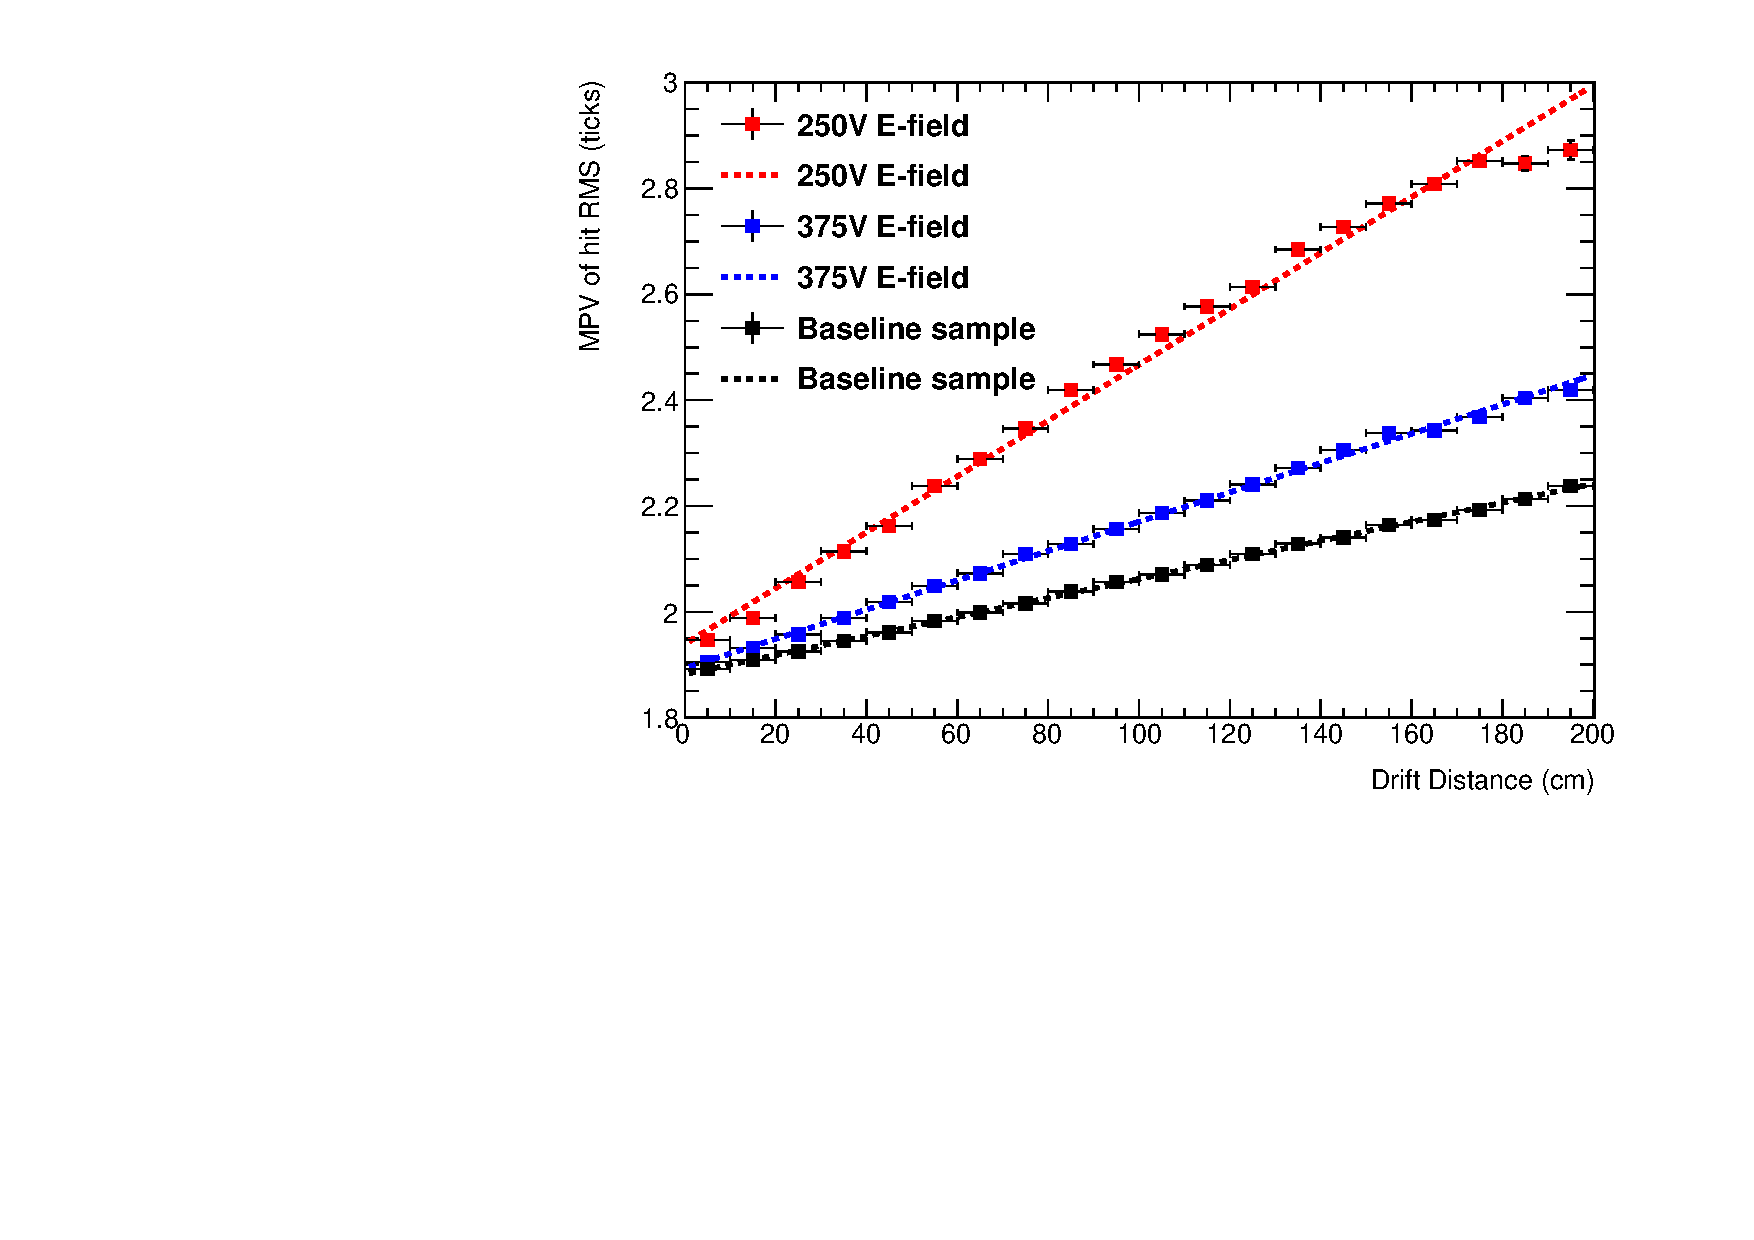
\includegraphics[width=0.6\textwidth]{Canvas_CountDiff4_All_Positions_ElecField}
    \caption[The most probable values of hit $RMS$ as a function of drift distance, for tracks associated with a coincidence that had a counter difference of 4, for different values of the electric field]
          {The most probable values of hit $RMS$ as a function of drift distance, for tracks associated with a coincidence that had a counter difference of 4, for different values of the electric field.}
  \label{fig:DiffElecStudy_CDiff4}
\end{figure}

\begin{figure}
  \centering
  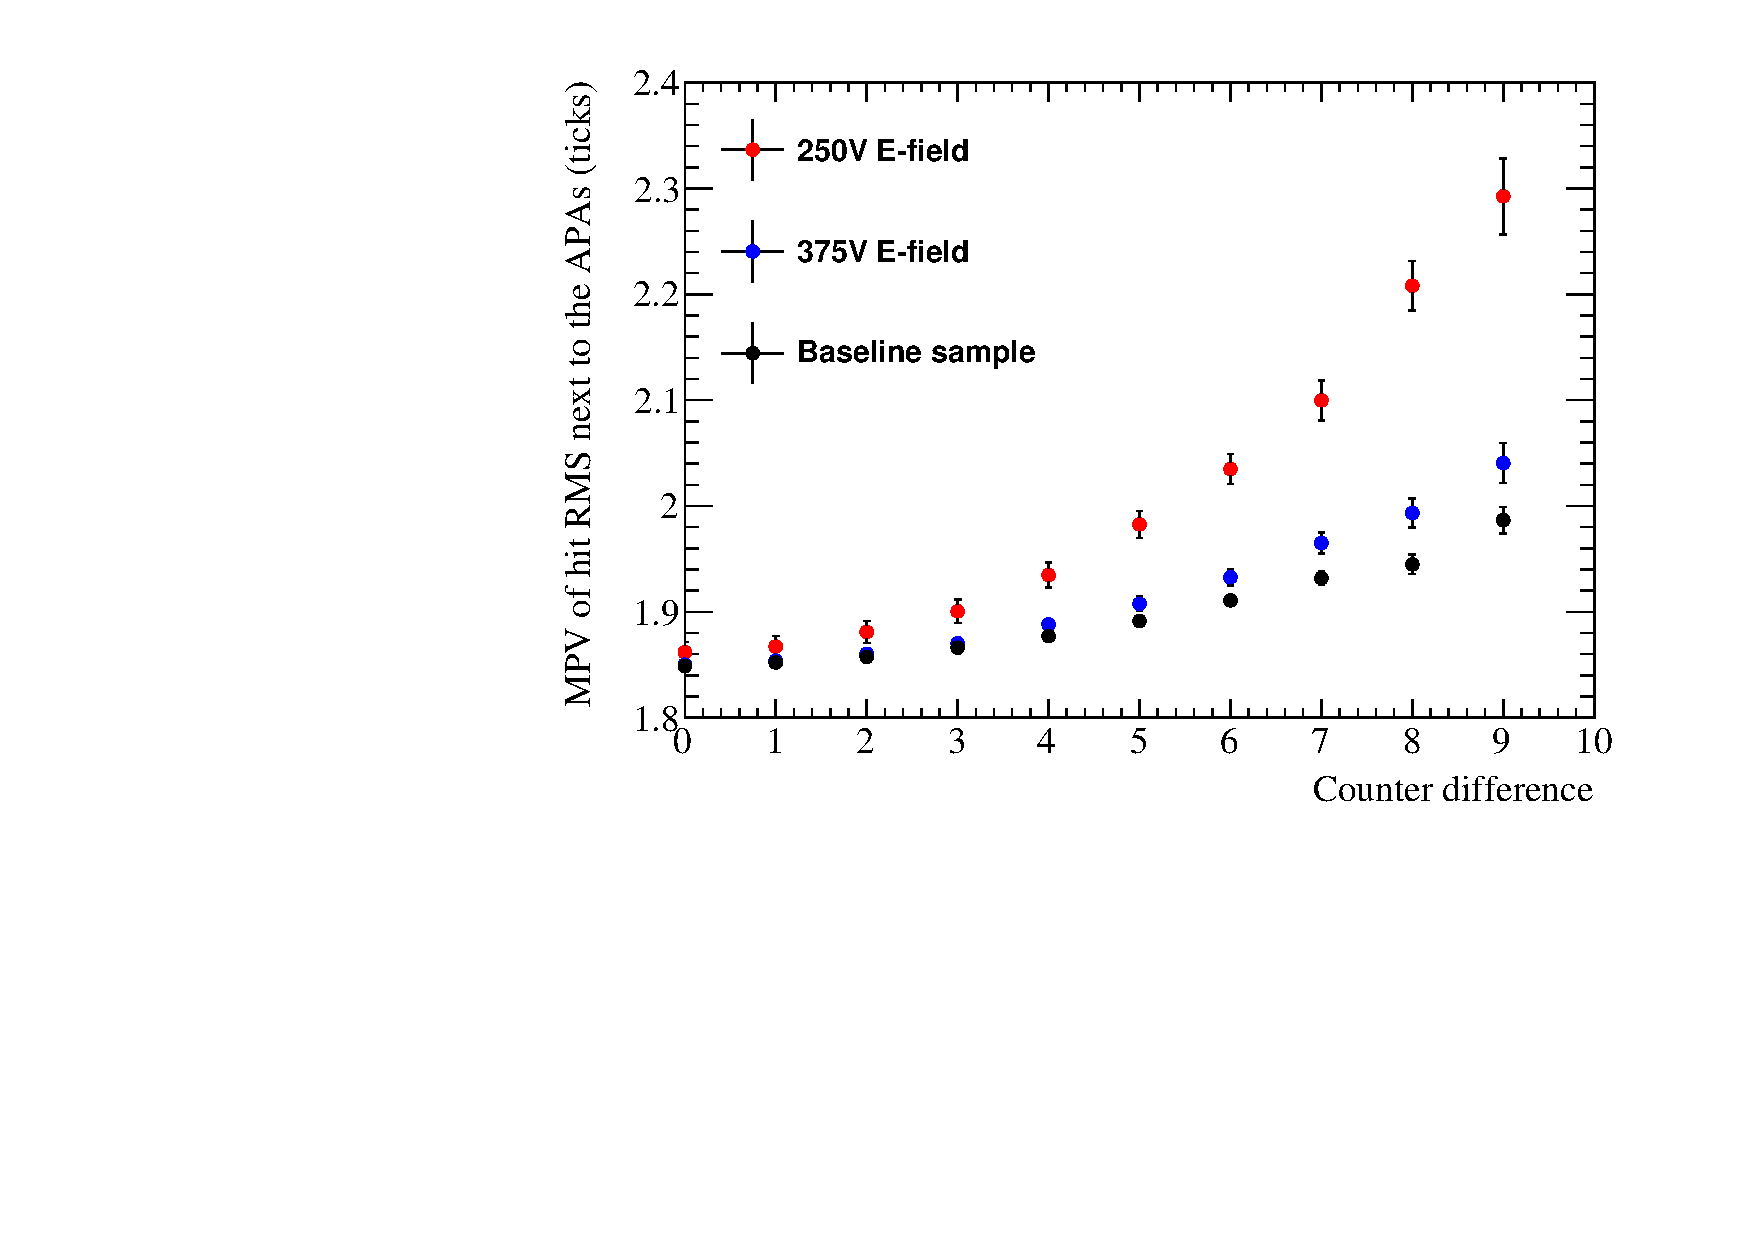
\includegraphics[width=0.6\textwidth]{Canvas_All_Angles_RMS0cm_ElecField}
  \caption[The angular dependence of hits within 10 cm of the APAs, for different values of the electric field]
          {The most probable values of hit $RMS$ within 10 cm of the APAs, as a function of the counter difference of the coincidence that the track was associated with, for different values of the electric field.}
  \label{fig:DiffElecStudy_RMS0cm}
\end{figure}

\begin{figure}
  \centering
  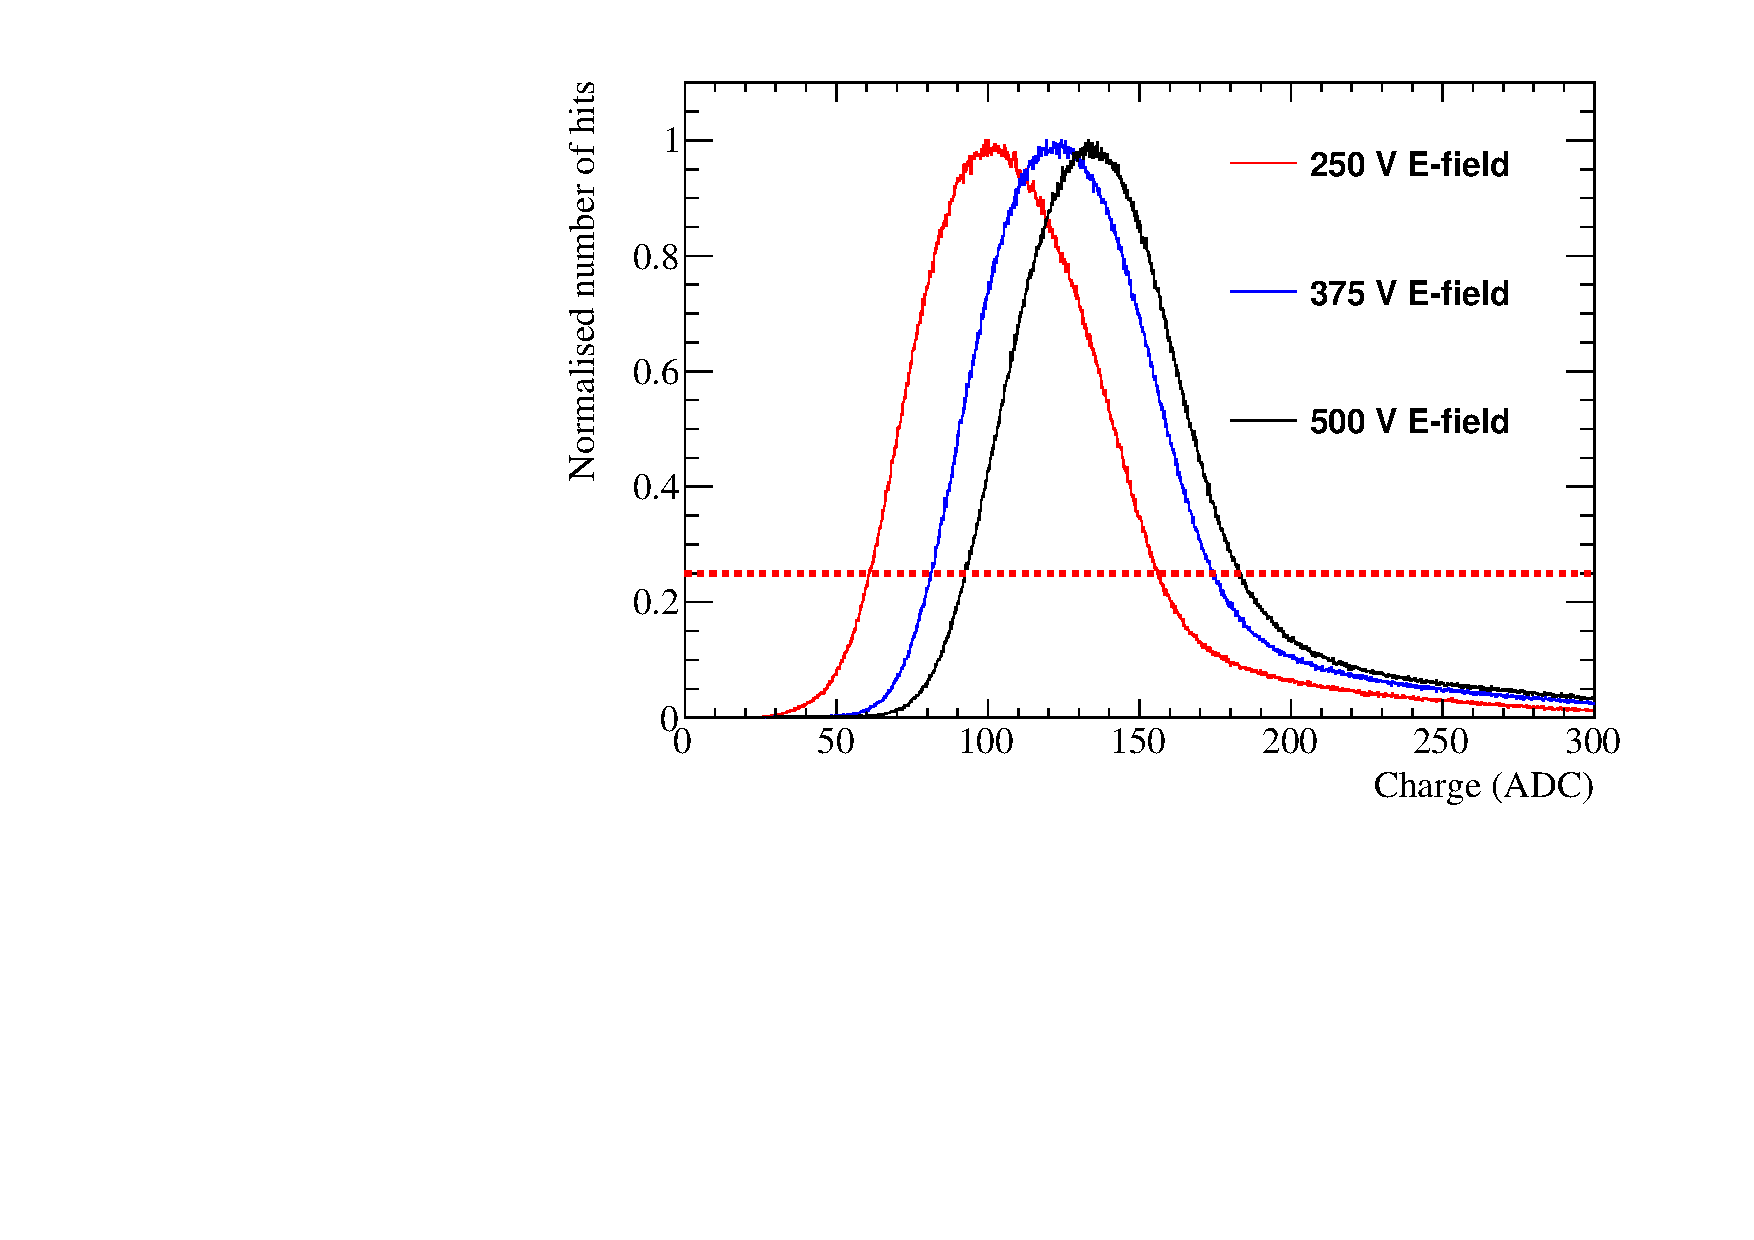
\includegraphics[width=0.6\textwidth]{Canvas_ChargeCut_ElecField}
  \caption[The normalised hit charge distribution for different values of the electric field]
          {The normalised hit charge distribution for different values of the electric field. The hit charge is shown in units of ADC, and is normalised so that the most common hit charge has a value of 1. A cut on the normalised number of hits being greater than 0.25 is shown, the aim of this cut is to remove the tails of the hit charge distribution.}
  \label{fig:DiffElecStudy_ChargeCut}
\end{figure}

%%%%%%%% The diffusion constant study

\begin{figure}
  \centering
  \begin{subfigure}{0.48\textwidth}
    \centering
    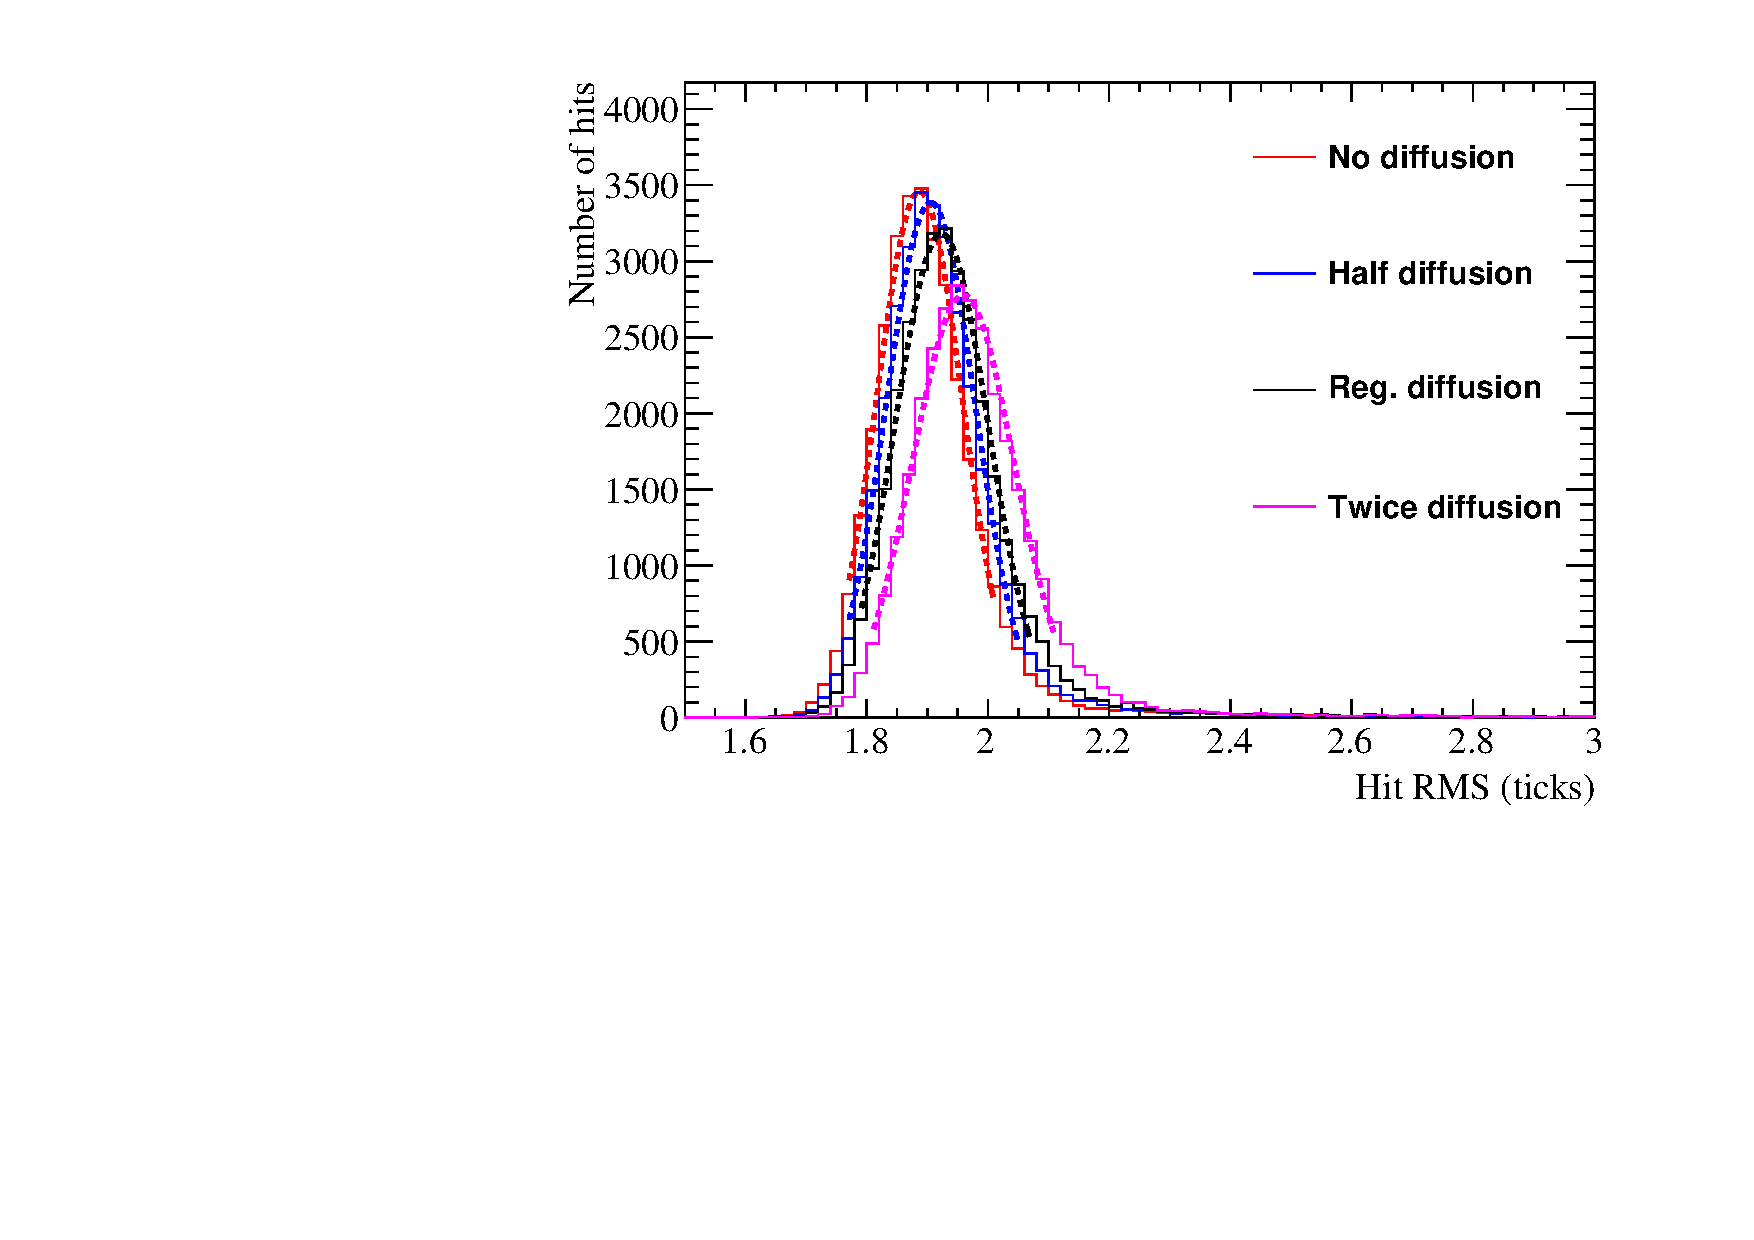
\includegraphics[width=\textwidth]{Canvas_RMS_20cm_Diffusion}
    \caption{The most probable hit $RMS$ values for hits between $x =$ 20 cm and $x =$ 30 cm.}
  \end{subfigure}%
  \hspace{0.03\textwidth}%
  \begin{subfigure}{0.48\textwidth}
    \centering
    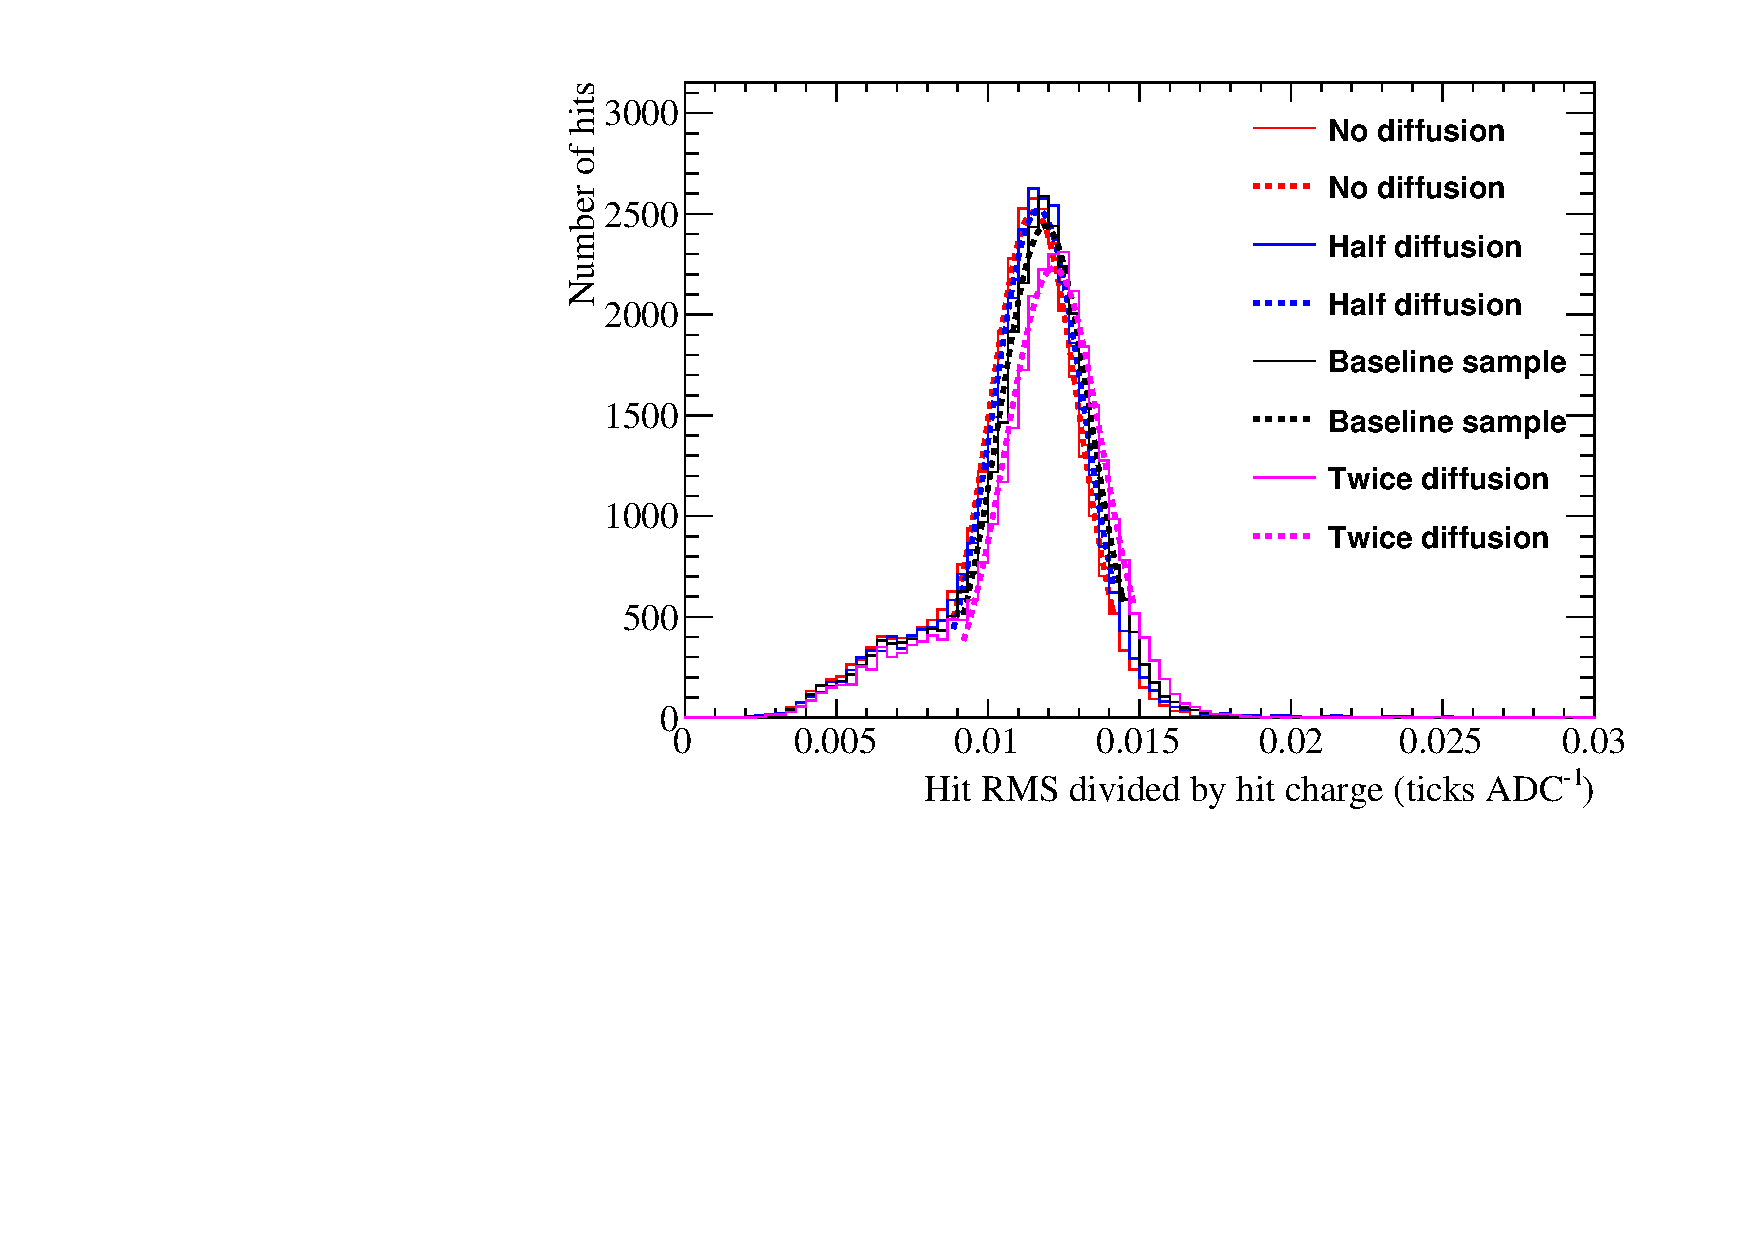
\includegraphics[width=\textwidth]{Canvas_RMS_Q_20cm_Diffusion}
    \caption{The most probably hit $RMS/Charge$ values for hits between $x =$ 20 cm and $x =$ 30 cm.}
  \end{subfigure}
  \caption[The distributions of the hit $RMS$ and hit $RMS/Charge$ values for tracks with a counter difference of 4, for different values of the constant of longitudinal diffusion]
          {The distributions of the hit $RMS$ and hit $RMS/Charge$ values for hits between $x$~=~20~cm and $x$~=~30~cm, for tracks with a counter difference of 4, for different values of the constant of longitudinal diffusion.}
  \label{fig:DiffLDiff_HitFit}
\end{figure}

\begin{figure}
  \centering
  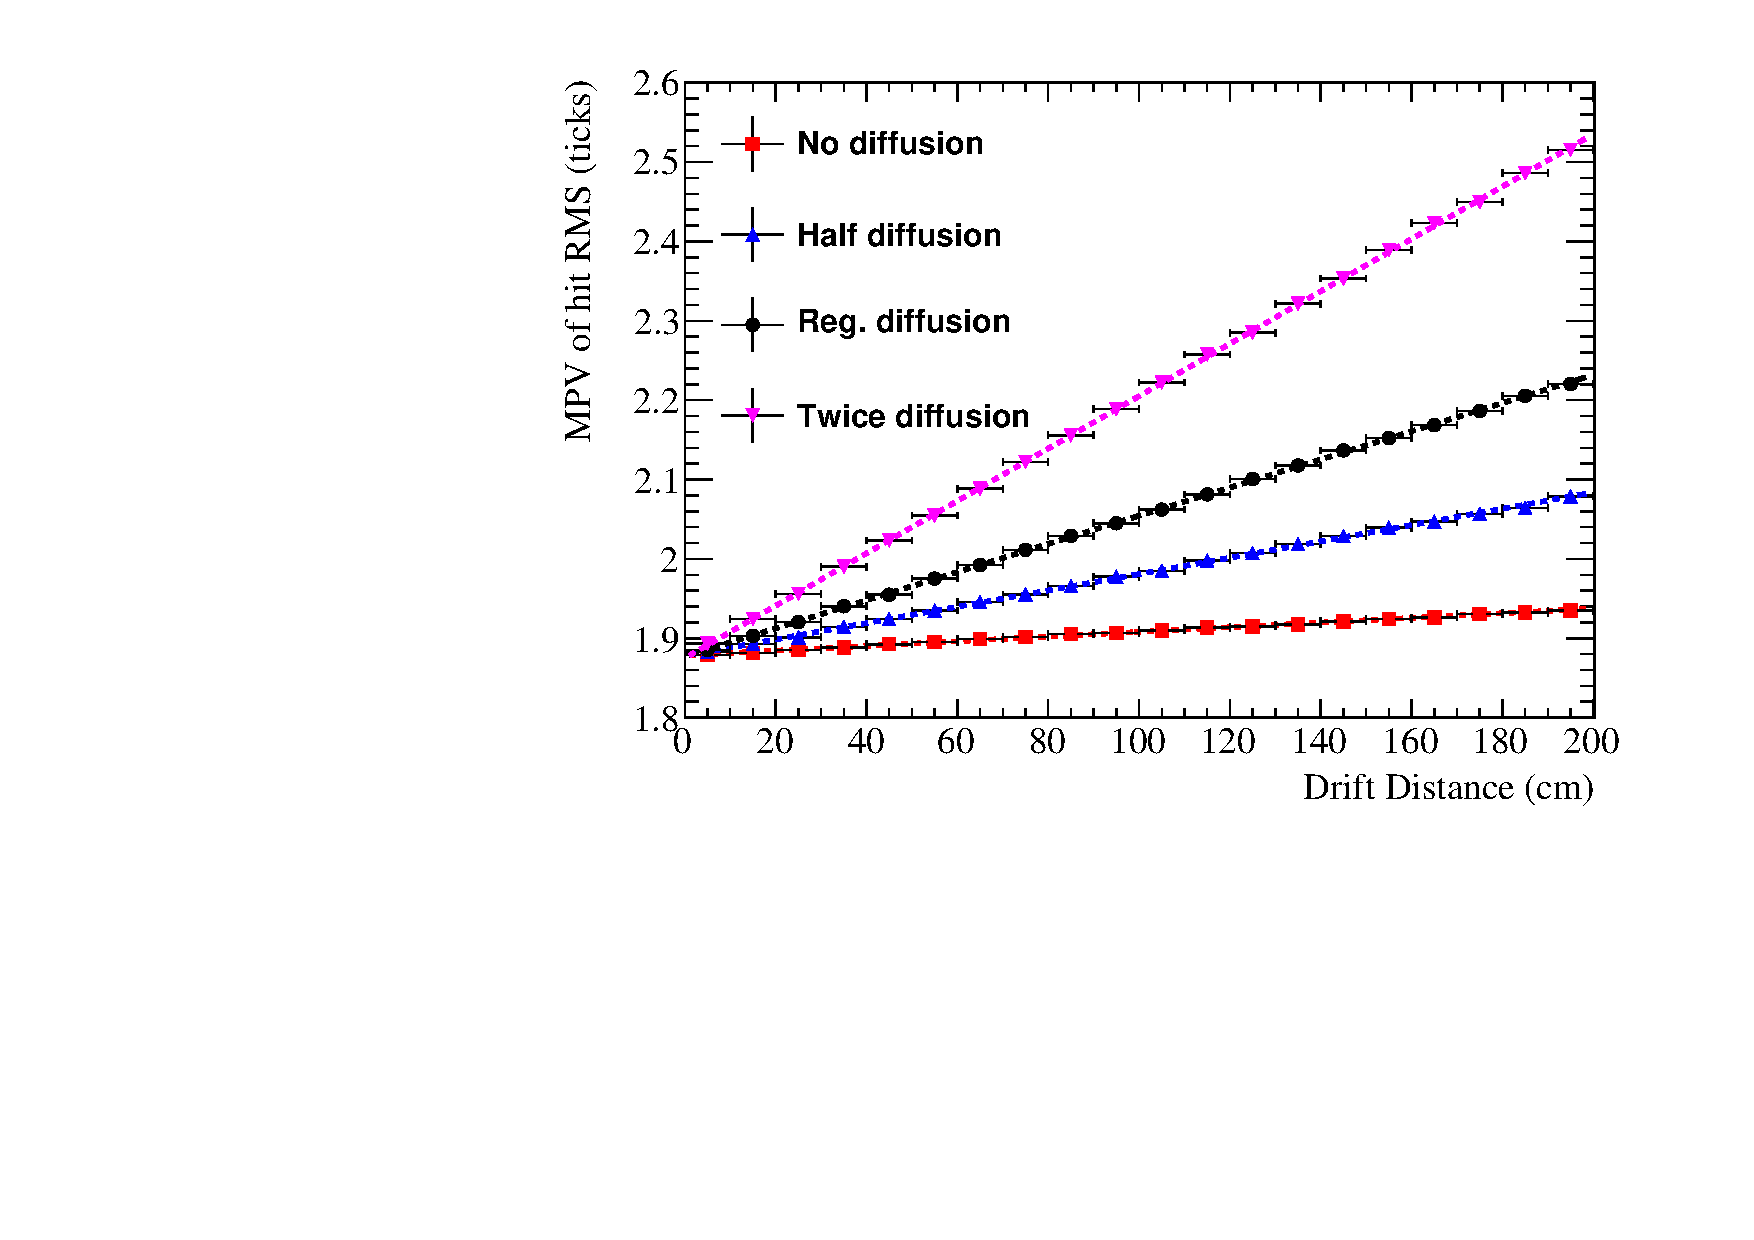
\includegraphics[width=0.6\textwidth]{Canvas_CountDiff4_All_Positions_Diffusion}
  \caption[The most probable values of hit $RMS$ as a function of drift distance, for tracks associated with a coincidence that had a counter difference of 4, for different values of the constant of longitudinal diffusion]
          {The most probable values of hit $RMS$ as a function of drift distance, for tracks associated with a coincidence that had a counter difference of 4, for different values of the constant of longitudinal diffusion.}
  \label{fig:DiffLDiff_CDiff4}
\end{figure}

\begin{figure}
  \centering
  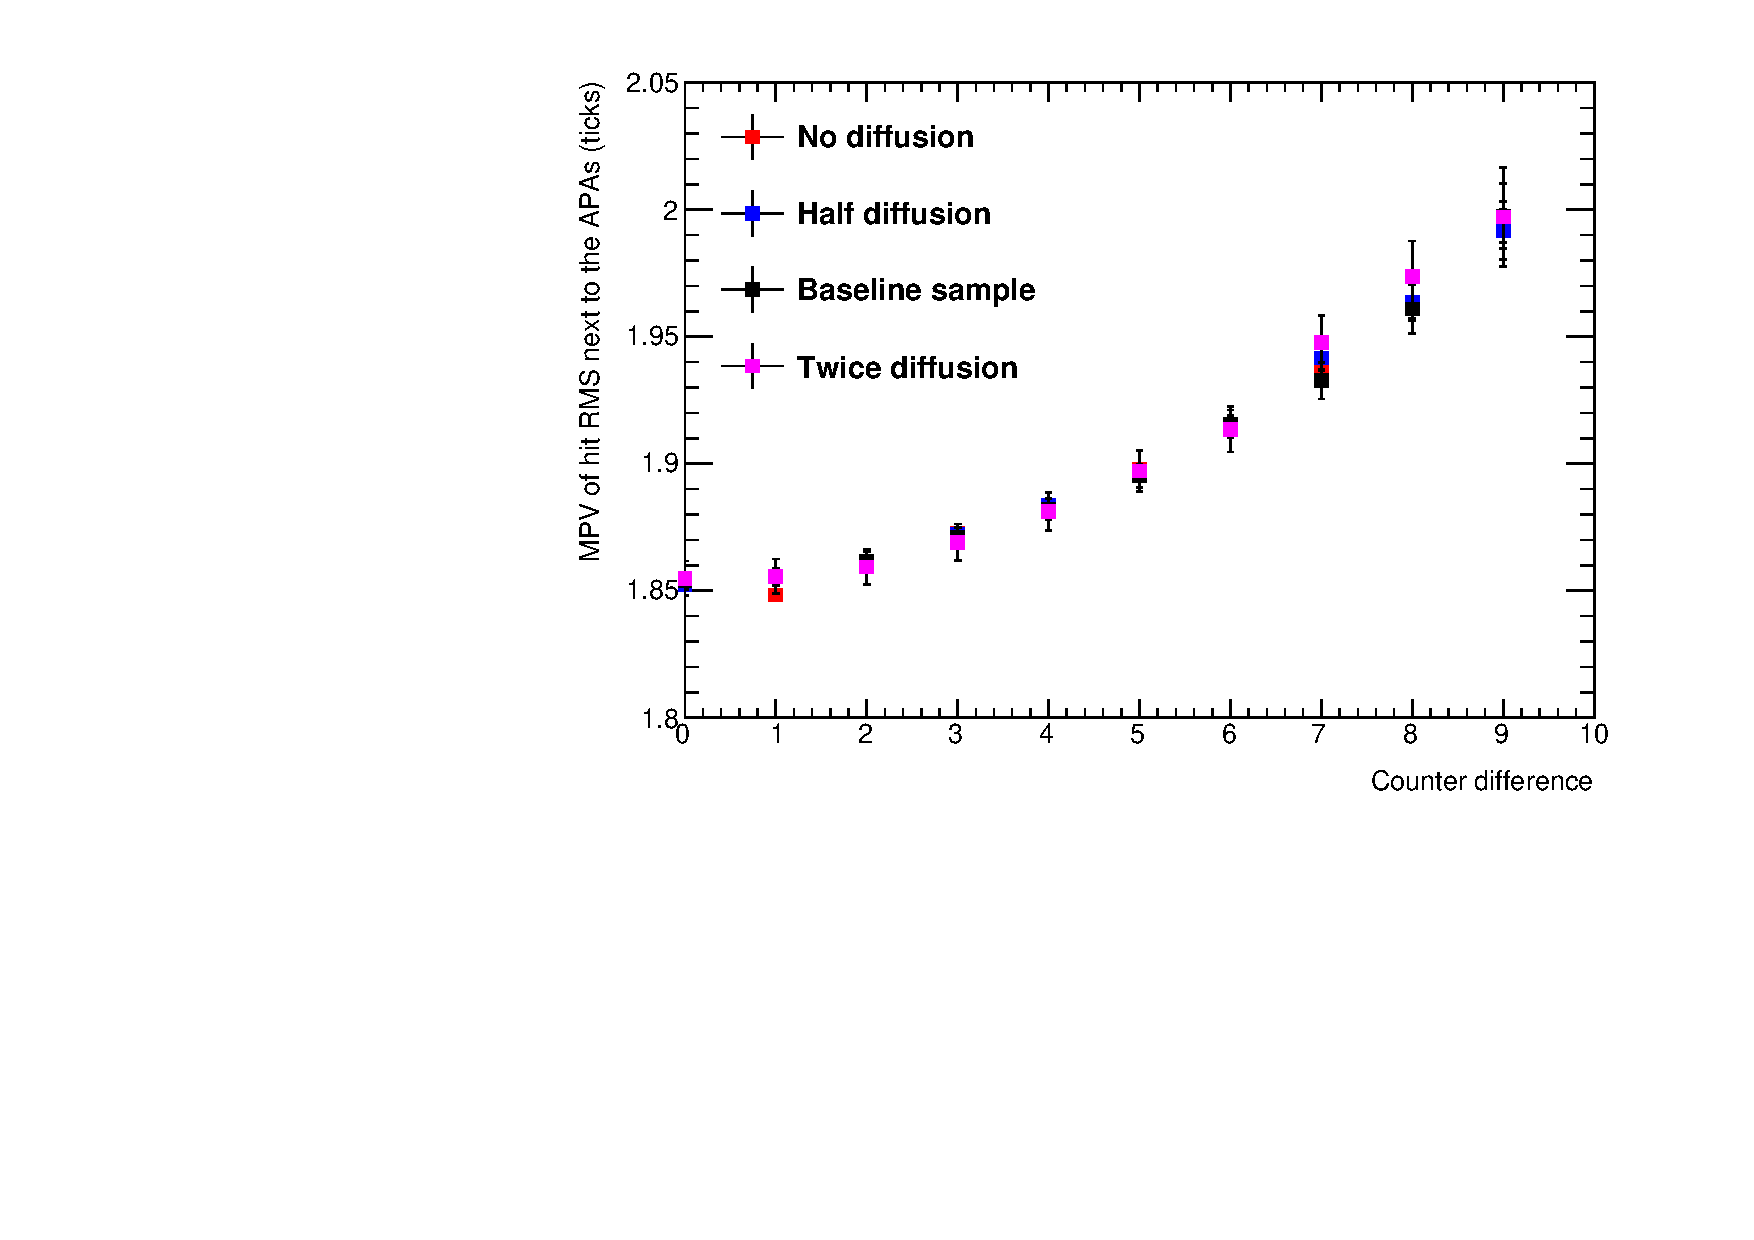
\includegraphics[width=0.6\textwidth]{Canvas_All_Angles_RMS0cm_Diffusion}
  \caption[The angular dependence of hits within 10 cm of the APAs, for different values of the constant of longitudinal diffusion]
          {The most probable values of hit $RMS$ within 10 cm of the APAs, as a function of the counter difference of the coincidence that the track was associated with, for different values of the constant of longitudinal diffusion.}
  \label{fig:DiffLDiff_RMS0cm}
\end{figure}

\begin{figure}
  \centering
  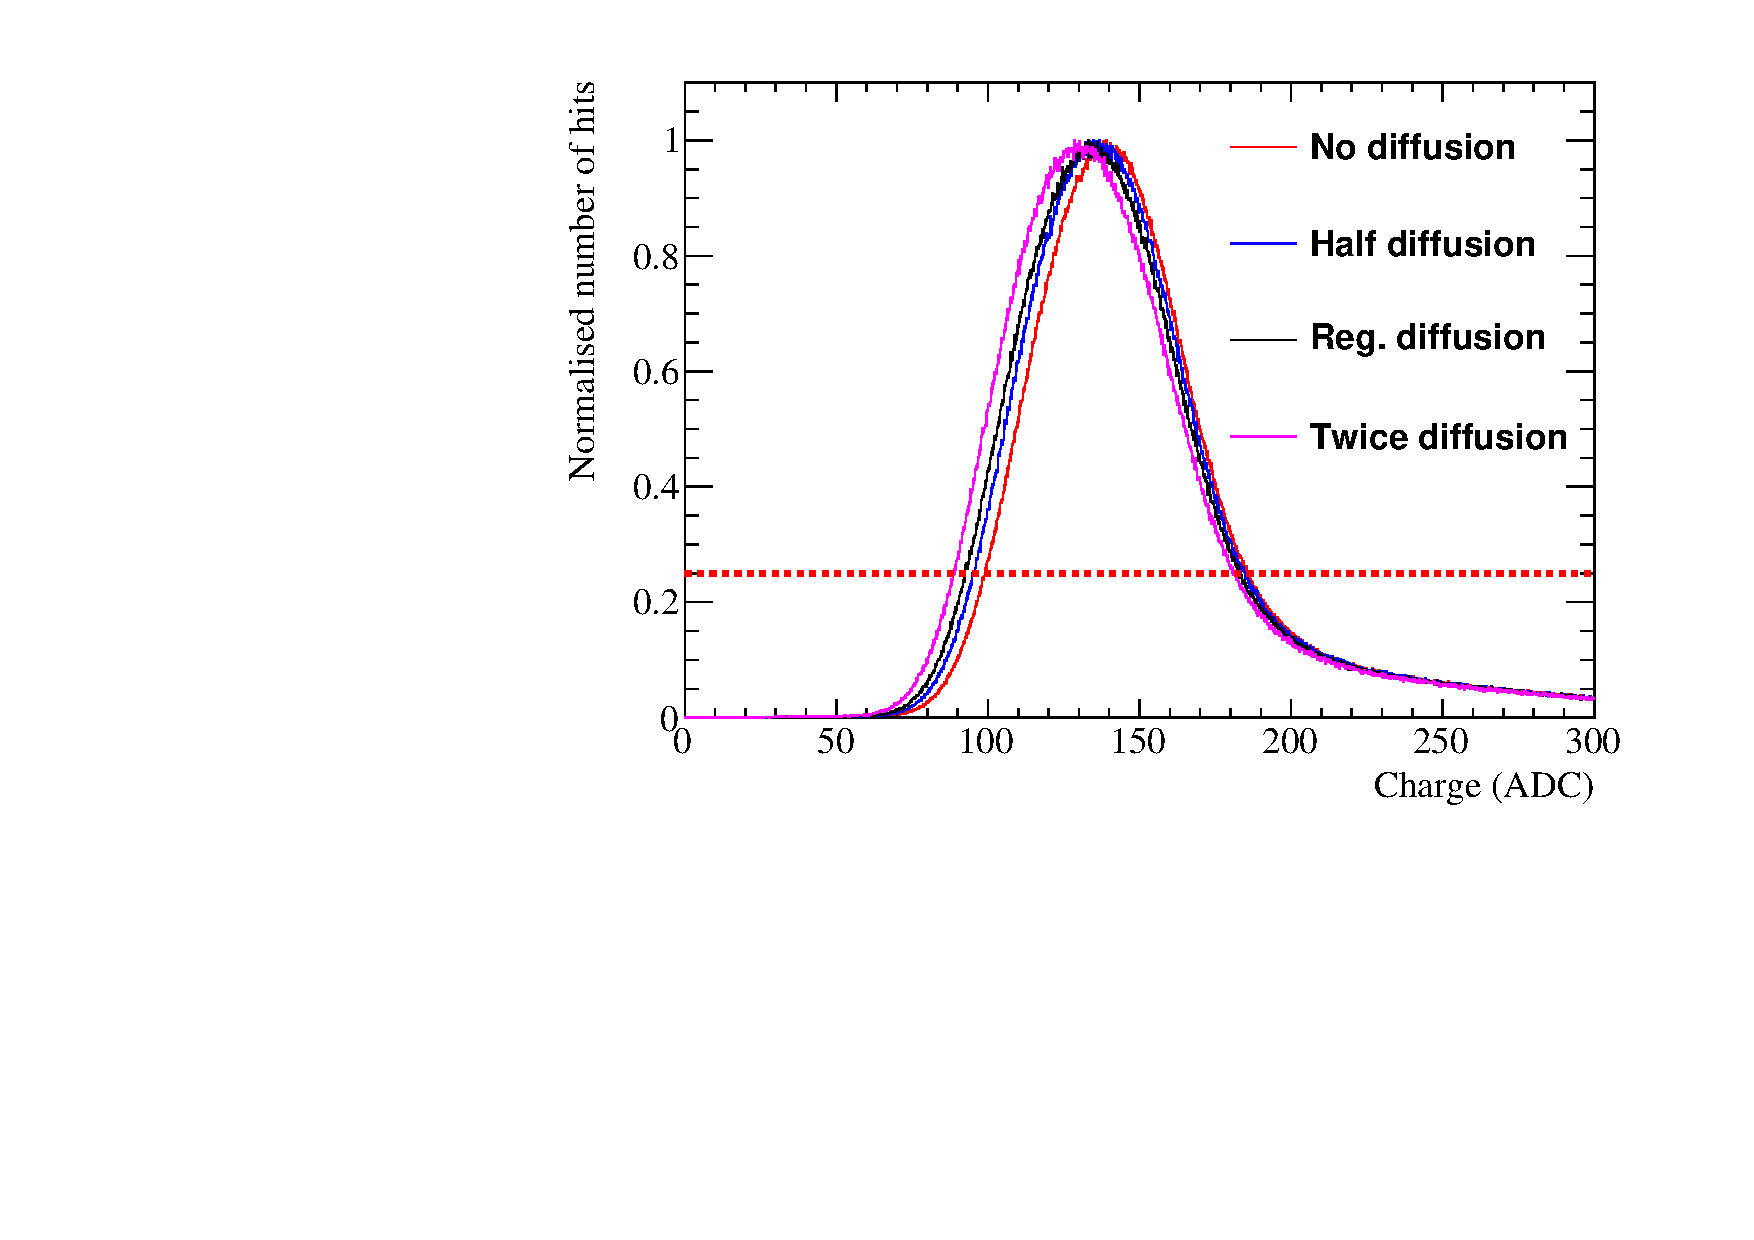
\includegraphics[width=0.6\textwidth]{Canvas_ChargeCut_Diffusion}
  \caption[The normalised hit charge distribution for different values of the constant of longitudinal diffusion]
          {The normalised hit charge distribution for different values of the constant of longitudinal diffusion. The hit charge is shown in units of ADC, and is normalised so that the most common hit charge has a value of 1. A cut on the normalised number of hits being greater than 0.25 is shown, the aim of this cut is to remove the tails of the hit charge distribution.}
  \label{fig:DiffLDiff_ChargeCut}
\end{figure}
